% LunaStack 使い方ガイド（初心者向け）
%
% 組版: docs/manual で  latexmk  （設定は .latexmkrc。LuaLaTeX・jlreq・原ノ味フォント）
% 図:   tools/make_shots.sh でアプリの画面を撮り、tools/figures.py で figures/ を作る
\documentclass[paper=a4,fontsize=10.5pt,report,line_length=44zw,number_of_lines=42,
  head_space=18mm,foot_space=14mm]{jlreq}
\usepackage{lsmanual}
\usepackage{luatexja-fontspec}
\usepackage{amsmath}
\usepackage{multicol}
\usepackage[hidelinks,bookmarksnumbered,pdftitle={LunaStack 使い方ガイド},pdfauthor={LunaStack}]{hyperref}
\captionsetup{font=small,labelsep=quad}
\setcounter{tocdepth}{1}

\newcommand{\LS}{LunaStack}
\newcommand{\version}{1.0.0}

\begin{document}

% ---- 表紙 ----------------------------------------------------------------------
\begin{titlepage}
  \begin{tikzpicture}[remember picture, overlay]
    \fill[lsnight] (current page.north west) rectangle (current page.south east);
    \foreach \i in {1,...,160} {
      \pgfmathsetmacro{\x}{rnd*21}\pgfmathsetmacro{\y}{rnd*29.7}\pgfmathsetmacro{\r}{0.2+rnd*0.9}
      \fill[white, opacity=0.35+0.5*rnd] ($(current page.south west)+(\x cm,\y cm)$) circle (\r pt);
    }
    \node[anchor=center] at ($(current page.center)+(0,3.2cm)$) {%
      \begin{tikzpicture}
        \shade[ball color=yellow!15!white] (0,0) circle (2.4cm);
        \fill[lsnight, opacity=0.92] (0.9,0.25) circle (2.35cm);
      \end{tikzpicture}};
    \node[text=white, font=\sffamily\bfseries\fontsize{40}{46}\selectfont] at ($(current page.center)+(0,-1.6cm)$) {\LS};
    \node[text=white, font=\sffamily\Large] at ($(current page.center)+(0,-3.0cm)$) {使い方ガイド};
    \node[text=white!75, font=\sffamily\normalsize, align=center] at ($(current page.center)+(0,-4.6cm)$)
      {月・惑星のスタック処理を、はじめての人にも};
    \node[text=white!60, font=\sffamily\small] at ($(current page.south)+(0,2.5cm)$)
      {バージョン \version\quad macOS 10.13 以降};
  \end{tikzpicture}
\end{titlepage}

\tableofcontents

\chapter{\LS でできること}

\section{このソフトは何をするのか}

望遠鏡で月や惑星を撮ると、1枚だけではどうしてもぼやけた、ざらついた写真になります。原因はおもに2つです。

\begin{itemize}
  \item \textbf{大気のゆらぎ（シーイング）}：空気の温度むらがレンズのように働き、像が一瞬ごとにゆがんだり、にじんだりします。
        星がまたたくのと同じ現象です。
  \item \textbf{ノイズ}：暗い対象を短い露出で撮ると、画面がざらざらします。
\end{itemize}

そこで、\textbf{動画（または連続写真）で数百〜数千枚を撮り、写りのよい瞬間だけを選んで重ね合わせる}という方法がとられます。
これを\textbf{スタック（スタッキング）}と呼びます。重ねるほどノイズは減り、ゆらぎの少ない瞬間だけを使うので細部もくっきりします。
\LS は、この「選ぶ・位置を合わせる・重ねる・仕上げる」を1つのアプリで行うソフトです。

\begin{center}
\begin{tikzpicture}[font=\sffamily\small, >=Stealth]
  % 入力のフレーム
  \foreach \i/\s in {0/0.55,1/0.8,2/0.35,3/0.9,4/0.5} {
    \begin{scope}[shift={(\i*0.28,-\i*0.22)}]
      \fill[black!85, draw=white, line width=0.6pt] (0,0) rectangle (1.6,1.6);
      \shade[inner color=yellow!40!white, outer color=orange!60!black, opacity=\s] (0.8,0.8) circle (0.52);
    \end{scope}
  }
  \node[align=center, font=\sffamily\footnotesize] at (1.4,-1.75) {撮った動画\\（数百〜数千枚）};
  \draw[->, line width=1.4pt, lsgray] (3.2,0.2) -- (4.3,0.2);
  % 選別
  \begin{scope}[shift={(4.6,-0.6)}]
    \foreach \i/\ok in {0/1,1/0,2/1,3/0,4/1} {
      \fill[black!85] (\i*0.62,0) rectangle ++(0.54,0.54);
      \shade[inner color=yellow!40!white, outer color=orange!60!black, opacity=0.8] (\i*0.62+0.27,0.27) circle (0.18);
      \ifnum\ok=1 \draw[lsgreen, line width=1.2pt] (\i*0.62-0.03,-0.03) rectangle ++(0.60,0.60);
      \else \draw[lsred, line width=1.1pt] (\i*0.62+0.07,0.07) -- ++(0.4,0.4) (\i*0.62+0.47,0.07) -- ++(-0.4,0.4); \fi
    }
    \node[align=center, font=\sffamily\footnotesize] at (1.5,-0.95) {よく写った瞬間だけ選ぶ\\（品質評価）};
  \end{scope}
  \draw[->, line width=1.4pt, lsgray] (7.9,0.2) -- (9.0,0.2);
  % 位置合わせ・重ね合わせ
  \begin{scope}[shift={(9.3,-0.6)}]
    \fill[black!85] (0,0) rectangle (1.6,1.6);
    \shade[inner color=yellow!25!white, outer color=orange!70!black] (0.8,0.8) circle (0.55);
    \draw[orange!50!black, line width=0.7pt] (0.3,0.72) .. controls (0.8,0.62) .. (1.3,0.72);
    \draw[orange!50!black, line width=0.7pt] (0.3,0.95) .. controls (0.8,1.05) .. (1.3,0.95);
    \node[align=center, font=\sffamily\footnotesize] at (0.8,-0.95) {位置を合わせて重ねる\\（アライメント・スタック）};
  \end{scope}
  \draw[->, line width=1.4pt, lsgray] (11.2,0.2) -- (12.1,0.2);
  \begin{scope}[shift={(12.4,-0.6)}]
    \fill[black!85] (0,0) rectangle (1.6,1.6);
    \shade[inner color=white, outer color=orange!80!black] (0.8,0.8) circle (0.55);
    \draw[orange!40!black, line width=1.0pt] (0.28,0.72) .. controls (0.8,0.60) .. (1.32,0.72);
    \draw[orange!40!black, line width=1.0pt] (0.28,0.95) .. controls (0.8,1.07) .. (1.32,0.95);
    \fill[orange!70!black] (1.0,0.5) ellipse (0.12 and 0.07);
    \node[align=center, font=\sffamily\footnotesize] at (0.8,-0.95) {細部を引き出す\\（仕上げ）};
  \end{scope}
\end{tikzpicture}
\captionof{figure}{\LS の処理のイメージ}\label{fig:concept}
\end{center}

\section{処理の流れ}

\LS の処理は、次の6つの段階に分かれています。画面の下にある4つのボタン \ui{品質評価}\ui{アライメント}\ui{スタック}\ui{書き出し…}
が、ちょうどこの流れに対応しています。\textbf{各段階が終わるとアプリはいったん止まり}、結果を確かめてから次へ進めます。

\begin{center}
\begin{tikzpicture}[font=\sffamily\small, node distance=3mm,
    st/.style={draw=lsnight, fill=lspale, rounded corners=3pt, minimum height=11mm, text width=21mm, align=center, line width=0.8pt, font=\sffamily\footnotesize},
    ar/.style={-{Stealth[length=2.5mm]}, line width=1.1pt, lsnight}]
  \node[st] (a) {① 追加\\{\scriptsize 動画・写真}};
  \node[st, right=of a] (b) {② 品質評価\\{\scriptsize 写りを採点}};
  \node[st, right=of b] (c) {③ アライメント\\{\scriptsize 位置を合わせる}};
  \node[st, right=of c] (d) {④ スタック\\{\scriptsize 重ね合わせる}};
  \node[st, right=of d] (e) {⑤ 仕上げ\\{\scriptsize シャープ・色}};
  \node[st, right=of e] (f) {⑥ 書き出し\\{\scriptsize ファイルに保存}};
  \foreach \p/\q in {a/b,b/c,c/d,d/e,e/f} \draw[ar] (\p) -- (\q);
  \draw[ar, lsorange, dashed] (d.south) .. controls +(0,-0.9) and +(0,-0.9) .. node[below, font=\sffamily\scriptsize, text=lsorange!80!black]
    {採用率だけ変えるなら解析はやり直さない} (d.south west);
\end{tikzpicture}
\captionof{figure}{処理の6段階}\label{fig:flow}
\end{center}

\begin{point}[この説明書の進め方]
  はじめての人は、まず\textbf{第\ref{chap:quickstart}章「はじめての処理」}をアプリを動かしながら読んでください。
  木星の動画を例に、追加から書き出しまでを一通り体験できます。設定の意味や数値の決め方は、第\ref{chap:quality}章〜第\ref{chap:finish}章で
  タブごとに詳しく説明します。うまくいかないときは第\ref{chap:trouble}章を見てください。
\end{point}

\section{覚えておきたい言葉}

この説明書とアプリの画面に出てくる言葉です。いまは全部覚えなくてもかまいません。

\begin{description}[style=nextline, leftmargin=1.5em, font=\sffamily\bfseries, itemsep=0.35em]
  \item[フレーム] 動画の1コマ（または連続写真の1枚）。
  \item[品質・品質評価] フレームごとの「写りのよさ」の点数。細かい模様がくっきり写っているほど高くなります。
  \item[参照画像] 位置合わせの「お手本」になる画像。品質の高いフレームをいくつか平均して作ります。
  \item[アライメント（位置合わせ）] 各フレームのずれを測り、お手本に重なるように合わせること。
  \item[位置合わせ領域] 画像を小さな四角（数十画素）に分けたもの。大気のゆらぎは場所ごとにずれ方が違うので、
        \LS は四角ごとに別々に位置を合わせ、四角ごとに写りのよいフレームを選びます。他のソフトでは「AP（Alignment Point）」とも呼ばれます。
  \item[スタック] 選んだフレームを重ねて平均すること。ノイズが減ります。
  \item[採用率] 重ねるために使うフレームの割合（上位何\%か）。
  \item[ウェーブレット] 画像を「細かい模様」から「大きな模様」まで6段階（レイヤー）に分け、段階ごとに強調やノイズ低減をする仕上げの方法です。
  \item[ドリズル] 位置のずれを利用して、元より細かい画素で画像を作り直す拡大の方法。条件がそろったときだけ効果があります。
  \item[Bayer（ベイヤー）・デバイヤー] カラーカメラのセンサーは、画素ごとに赤・緑・青のどれか1色しか測っていません。
        この並びを Bayer 配列と呼び、各画素の3色をそろえる処理をデバイヤー（色補間）と呼びます。
  \item[サイドカー] 解析結果を保存したファイル（元ファイルの隣に \texttt{.lstk}・\texttt{.lstkq} という名前で自動で作られます）。
        同じファイルを開き直すと、この内容を読み込んで解析を省けます。
\end{description}

\section{動作環境と読めるファイル}

\begin{tabularx}{\linewidth}{@{}>{\sffamily\bfseries}l X@{}}
\toprule
動作環境 & macOS 10.13（High Sierra）以降。Intel と Apple シリコンのどちらの Mac でも動きます。\\
\midrule
動画 & SER、AVI（非圧縮・MJPEG）、MOV・MP4・M4V（H.264・HEVC・ProRes など）\\
静止画の連番 & TIFF、PNG、FITS、JPEG、カメラの RAW（CR2・CR3・NEF・ARW・RAF・ORF・RW2・PEF・DNG など）。
  フォルダごと、または複数の画像をまとめて追加すると、1本の「連番」として扱います。\\
書き出し & 16bit TIFF、32bit 浮動小数点 TIFF、32bit 浮動小数点 FITS、16bit PNG\\
\bottomrule
\end{tabularx}

\begin{tip}[おすすめの撮り方]
  惑星なら SER 形式（FireCapture・SharpCap などの撮影ソフトで選べます）の動画を1〜3分、数千フレーム撮るのがおすすめです。
  SER と AVI は \LS が自分で読むので、どの Mac でも同じ結果になります。MOV・MP4 は macOS の機能で読むため、
  macOS の版によって画素の値がわずかに変わることがあります（第\ref{sec:movie}節）。
\end{tip}

\section{この説明書の図の見方}

スクリーンショットには、赤い枠と番号 \badge{1}\,\badge{2}\,\badge{3} を付けてあります。図のすぐ下に、同じ番号で説明を並べています。
オレンジの太い矢印は「ドラッグ（押したまま動かす）」を表します。ボタンの名前は \ui{スタック}、画面上の文字は \uil{位置合わせ領域} のように書きます。
キーボードの操作は \key{⌘}\,\key{R}（command キーを押しながら R）のように書きます。

\chapter{画面の見方}\label{chap:screen}

\section{起動したところ}

\LS を起動すると、次のような画面が出ます。ウインドウは大きく\textbf{左・中央・右}の3つに分かれていて、下に工程のボタンが並びます。

\screen{win_empty}{起動した直後の画面}{%
  \mk{queue}{1}\mk[e]{addbutton}{2}\mk{graph}{3}\mkd[isw]{preview}{4}
  \mk[w]{presets}{5}\mk[w]{tabs}{6}\mkd[w]{inspector}{7}\mk[nw]{process}{8}\mk[w]{status}{9}
  \drag{(0.47,0.60)}{($(queue-e)+(0.004,0)$)}
  \node[lscallout] at (0.47,0.66) {Finder から動画やフォルダを\\ここへドラッグ＆ドロップ};}

\begin{marklist}
  \item \textbf{入力キュー}：処理するファイルの一覧です。ここへファイルやフォルダを\textbf{ドラッグ＆ドロップ}して追加できます。
  \item \ui{追加…}：ファイルを選んで追加します（メニューの「ファイル → 開く…」\key{⌘}\key{O} と同じ）。
        \ui{削除} は選んだファイルを一覧から外し、\ui{クリア} は一覧・結果・設定をすべて初期状態に戻します（元のファイルは消えません）。
  \item \textbf{品質グラフ}：品質評価をすると、フレームごとの点数がここにグラフで出ます。
  \item \textbf{プレビュー}：いま扱っている画像を大きく表示します。
  \item \textbf{プリセット}：すべての設定をひとまとめにして保存・読み込みします（第\ref{sec:preset}節）。
  \item \textbf{工程タブ}：右側の設定を「品質評価・アライメント・スタック・仕上げ・出力」の4つに分けています。
        工程が終わると次のタブへ自動で切り替わります。
  \item \textbf{設定パネル}：いまのタブの設定が並びます。上下にスクロールできます。
  \item \textbf{工程のボタン}：\ui{品質評価}\ui{アライメント}\ui{スタック}\ui{書き出し…}。前の工程が終わるまでは押せません（灰色）。
  \item \textbf{状態表示}：いま何をしているか、次に何をすればよいかが出ます。処理中は進み具合と残り時間、\ui{中断} ボタンが出ます。
\end{marklist}

\section{処理したあとの画面}

スタックと仕上げまで終えると、画面の各部にいろいろな情報が出ます。

\screen{win_overview}{スタックと仕上げを終えた画面}{%
  \mk{queue}{1}\mk{graph}{2}\mkd[inw]{preview}{3}\mk[nw]{viewmode}{4}\mk[s]{frameslider}{5}\mk[sw]{zoom}{6}\mk[s]{display}{7}
  \mk[nw]{banner}{8}\mk[w]{tabs}{9}\mkd[w]{inspector}{10}\mk[s]{process}{11}\mk[w]{status}{12}}

\begin{marklist}
  \item 入力キューの各行には、ファイル名と「フレーム数・画像の大きさ・形式」、処理の段階（\uil{未処理}\uil{品質評価済}\uil{アライメント済}\uil{完了}）が出ます。
  \item 品質グラフ：オレンジの横線は「参照画像に使う上位の割合」です（第\ref{sec:qs-quality}節）。
  \item プレビュー：スタックの結果（仕上げを掛けたもの）が出ています。
  \item 表示の切り替え：\uil{フレーム}（撮った1コマ）、\uil{参照}（位置合わせのお手本）、\uil{結果}（スタックの結果）。
  \item フレーム送り：スライダーと \ui{←}\ui{→} で、表示するフレームを選びます。
  \item 拡大率：\uil{全体}（ウインドウに合わせる）、\uil{100\%}（画面の画素と1対1）、\uil{200\%}、\uil{400\%}。
  \item \ui{表示} メニューと \uil{配置を編集}：位置合わせ領域の枠の表示、品質による色分け、画面だけ明るくする表示を切り替えます。
  \item 警告の帯：注意すべきことがあると、プレビューの上に出ます。\ui{×} で閉じられます（第\ref{chap:trouble}章）。
  \item 工程タブ：このときは「仕上げ・出力」が選ばれています。
  \item 設定パネル：仕上げの設定が並んでいます。
  \item 工程のボタン：一度実行すると \ui{品質を再評価}\ui{再アライメント}\ui{再スタック} に名前が変わります。
  \item 状態表示：最後の処理の結果（ここでは RGB のずれの量）が出ます。
\end{marklist}

\section{プレビューの下の道具}\label{sec:toolbar}

\screen{toolbar}{プレビューの下の道具}{%
  \mk[n]{viewmode}{1}\mk[n]{order}{2}\mk[n]{slider}{3}\mk[n]{step}{4}\mk[n]{info}{5}
  \mk[s]{zoom}{6}\mk[s]{display}{7}\mk[s]{apedit}{8}\mk[s]{apcount}{9}}

\begin{marklist}
  \item \textbf{表示の切り替え}：\uil{フレーム}・\uil{参照}・\uil{結果}。参照は品質評価のあと、結果はスタックのあとに選べます。
  \item \textbf{並び順}：スライダーでフレームを送る順番。\uil{時系列}（撮った順）と\uil{品質順}（写りのよい順）があります。
        品質評価のあとは品質順にすると、左端が最良、右へ行くほど悪いフレームになり、見比べやすくなります。
  \item \textbf{フレームのスライダー}：ドラッグしてフレームを選びます。
  \item \textbf{コマ送り}：\ui{←}\ui{→} で1枚ずつ送ります。押し続けると連続して送ります。キーボードの \key{←}\key{→} も使え、
        \key{shift} を押しながらだと10枚、\key{option} を押しながらだと100枚ずつ進みます。
  \item \textbf{表示中の画像の情報}：フレームなら「\#番号 / 総数・上位何\%・品質」、ほかに「参照画像」「スタック結果」など。
  \item \textbf{拡大率}：\key{⌘} を押しながらマウスのホイール、またはトラックパッドのピンチでも拡大・縮小できます（カーソルの位置が中心）。
        拡大しているときは2本指のスクロール（ホイール）で見る場所を動かせます。
  \item \ui{表示} メニュー：\uil{位置合わせ領域を表示}（枠の表示）、\uil{品質で色分け}（第\ref{sec:heatmap}節）、
        \uil{表示を明るくする（保存には影響しません）}（暗い画像を画面の上でだけ明るく見せる）。
  \item \uil{配置を編集}：オンにすると、プレビューをクリックして位置合わせ領域を足したり、選んで \key{delete} で消したりできます（第\ref{sec:apedit}節）。
  \item 位置合わせ領域の数と大きさ（例：\uil{位置合わせ領域 110 個 / 48 px}）。
\end{marklist}

\begin{tip}[画素の値を見る]
  プレビューの上にマウスを置くと、プレビューの下の道具の右端（位置合わせ領域の数の右）に、カーソル位置の座標と画素の値（0〜1）が出ます。
  白飛び（1.0 に張り付く）や黒つぶれを確かめるのに便利です。
\end{tip}

\section{設定パネルの使い方}

右の設定パネルは、\textbf{見出し}（\uil{▼ 各フレームの品質評価} のような太字の行）ごとにまとまっています。
見出しをクリックすると、その欄を\textbf{たたむ}（▶）・\textbf{開く}（▼）を切り替えられます。
ふだん触らない設定（\uil{詳細設定}など）はたたんでおくと見やすくなります。開閉の状態は次に起動したときも保たれます。

\begin{caution}[起動するたびに設定は初期値に戻ります]
  \LS は、起動するたびに入力キュー・設定・仕上げをすべて初期値から始めます（同じ条件を毎回確実に再現するため）。
  よく使う設定は\textbf{プリセット}に保存しておき、読み込んで使ってください（第\ref{sec:preset}節）。
  なお、解析済みのファイルを開いたときは、解析結果を使い回すのに必要な設定だけはサイドカーから戻ります。
\end{caution}

\section{左右の欄を隠す}

プレビューを広く使いたいときは、メニューの「表示」から左右の欄を隠せます。\key{⌘}\key{1} で左（入力キューと品質グラフ）、
\key{⌘}\key{2} で右（設定パネル）を、隠す・出すを切り替えます。

\chapter{はじめての処理 ——木星の動画を仕上げる}\label{chap:quickstart}

この章では、木星を撮った SER 動画（448×448 画素・カラー）を例に、追加から書き出しまでを一通り行います。
\textbf{設定はすべて初期値のままで}進めます。まずは流れをつかみ、設定の意味は後の章で確かめてください。

\begin{point}[この章の手順の早見表]
  \begin{enumerate}[label=\arabic*., itemsep=0pt, topsep=2pt]
    \item 動画を入力キューへドラッグ＆ドロップ
    \item \ui{品質評価} → 品質グラフとフレームを確認
    \item \ui{アライメント} → 参照画像と位置合わせ領域を確認
    \item \ui{スタック} → 結果を確認
    \item 「仕上げ・出力」タブでウェーブレットなどを調整
    \item \ui{書き出し…} でファイルに保存
  \end{enumerate}
\end{point}

% ------------------------------------------------------------------------------
\section{動画を追加する}\label{sec:qs-add}

\begin{step}{1}{動画を入力キューに入れる}
  Finder から動画ファイルを、左上の入力キューへドラッグ＆ドロップします。\ui{追加…} を押して選んでもかまいません。
\end{step}

\screen{qs_added}{動画を追加したところ}{%
  \mk[sw]{addbutton}{1}\mk{queuerow}{2}\mkd[inw]{preview}{3}\mk[s]{slider}{4}\mk[se]{framelabel}{5}
  \mk[nw]{quality}{6}\mk[w]{status}{7}\mk[w]{metric}{8}
  \drag{(0.30,0.93)}{($(queuerow-e)+(0.004,0)$)}\node[lscallout, anchor=west] at (0.31,0.93) {ドラッグ＆ドロップで追加};}

\begin{marklist}
  \item \ui{追加…}：ここから追加することもできます。
  \item 追加したファイル。副題に「4617 フレーム・448×448・SER v3」のように、フレーム数・大きさ・形式が出ます。状態は\uil{未処理}です。
  \item 1枚目のフレームが表示されます。まだぼやけていて、ざらざらしているのが分かります。
  \item スライダーで、ほかのフレームを見られます。
  \item いま表示しているフレームの番号（\uil{\#1 / 4617}）。
  \item \ui{品質評価} が押せるようになりました。
  \item ファイルの読み方の情報（ここではバイトオーダー）。
  \item 右の設定パネルは「品質評価」タブです。初期値のままでかまいません。
\end{marklist}

\begin{tip}[フォルダごと追加する]
  静止画（TIFF・PNG・JPEG・FITS・カメラの RAW）はフォルダごとドロップすると、中の画像を名前の順に並べた\textbf{1本の連番}として追加されます。
  複数の画像を選んでドロップしても、フォルダごとに1本にまとまります。
\end{tip}

% ------------------------------------------------------------------------------
\section{品質評価 ——写りのよいフレームを探す}\label{sec:qs-quality}

\begin{step}{2}{\ui{品質評価} を押す}
  画面左下の \ui{品質評価} を押します（\key{⌘}\key{E} でも同じ）。全フレームの「写りのよさ」を採点します。
  この 4617 フレームの動画で、10 秒ほどでした（2019 年の Intel Core i9 の MacBook Pro での例。古い Mac ではもっとかかります）。終わると「アライメント」タブに切り替わって止まります。
\end{step}

\screen{qs_quality}{品質評価が終わったところ}{%
  \mk{graph}{1}\mk[e]{cutline}{2}\drag{($(cutline-e)+(-0.03,0.02)$)}{($(cutline-e)+(-0.03,0.14)$)}
  \mk[n]{graphmode}{3}\mk[s]{slider}{4}\mk[se]{framelabel}{5}\mk[w]{tabs}{6}\mk[w]{method}{7}\mk[w]{refslider}{8}\mk[n]{align}{9}}

\begin{marklist}
  \item \textbf{品質グラフ}：縦が品質（上ほどよい）、横がフレームです。品質順に並べると、左端が最良、右端が最悪です。
        \textbf{この例では、左端に細い線が飛び出し、ほかのフレームは下に押しつぶされています}（下の注意を見てください）。
  \item \textbf{オレンジの線}：品質の上位何\%を\textbf{参照画像（お手本）}に使うかを示します（初期値は上位25\%）。
        線を上下にドラッグすると割合を変えられます。右の \badge{8} のスライダーと連動します。
  \item \uil{時系列}／\uil{品質順}：グラフの横軸を、撮った順と品質の順で切り替えます。
  \item プレビューのスライダーも品質順になりました。左端が品質の点数がいちばん高いフレームです。
  \item 表示中のフレームが全体の上位何\%か、元の番号、品質の値。
  \item 自動で「アライメント」タブに切り替わっています。
  \item 位置合わせの方法（初期値の\uil{複数領域の局所位置合わせ（推奨）}のままで）。
  \item 参照画像に使う割合のスライダー。
  \item \ui{アライメント} が押せるようになりました。
\end{marklist}

\begin{caution}[壊れたフレームが「最良」に見えることがある]
  \noindent
  \begin{minipage}[t]{0.26\linewidth}\vspace{0pt}\centering
    \shot[\linewidth]{graph_spikes}{\mk[ne]{spike}{1}}
  \end{minipage}\hfill
  \begin{minipage}[t]{0.33\linewidth}\vspace{0pt}\centering
    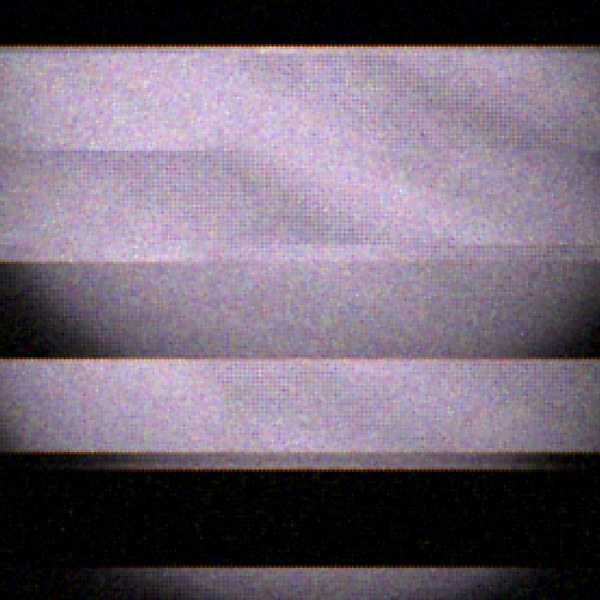
\includegraphics[width=\linewidth]{figures/frame_broken}\\[-1pt]
    {\scriptsize 点数がいちばん高かった「フレーム」}
  \end{minipage}\hfill
  \begin{minipage}[t]{0.36\linewidth}\vspace{0pt}
    この動画には、縞状に乱れた\textbf{壊れたフレーム}が約30枚まじっています。壊れたフレームは模様が異常にくっきりして見えるため、
    品質の点数が飛び抜けて高くなり、時系列のグラフでは \badge{1} のように針のように飛び出します。

    \smallskip
    心配はいりません。\textbf{次のアライメントで、お手本と似ていないフレームとして自動で除外}され（除外した枚数は警告の帯に出ます）、
    グラフも見やすくなります。
  \end{minipage}
\end{caution}

\subsection*{グラフの読み方}

アライメントのあと（壊れたフレームが除外されたあと）の品質グラフは、次のようになります。表示を切り替えると、別のことが分かります。

\noindent
\begin{minipage}[t]{0.47\linewidth}\centering
  \shot[0.62\linewidth]{graph_order}{\mk[e]{cutline}{1}\mk[ne]{best}{2}\mk[nw]{worst}{3}}
  \captionof{figure}{品質順}\label{fig:graph-order}
\end{minipage}\hfill
\begin{minipage}[t]{0.47\linewidth}\centering
  \shot[0.62\linewidth]{graph_timeline}{\mk[e]{cutline}{1}\mk[n]{mode}{4}}
  \captionof{figure}{時系列}\label{fig:graph-timeline}
\end{minipage}

\begin{marklist}
  \item オレンジの線より上のフレームが、参照画像（お手本）の材料になります。
  \item 品質順の左端：いちばん写りのよいフレーム群です。
  \item 右端：写りの悪いフレームです。除外したフレームは、いちばん右にまとめて並びます。
  \item 時系列にすると、撮影中に品質がどう変わったかが分かります。途中で大きく落ちている所があれば、雲が通ったり、ピントがずれたりした可能性があります。
\end{marklist}

グラフをクリックすると、その位置のフレームがプレビューに出ます（緑の縦線が表示中のフレーム）。
採用されたフレームのうち、最良と最悪のものを並べると次のようになります。

\noindent
\begin{minipage}[t]{0.47\linewidth}\centering
  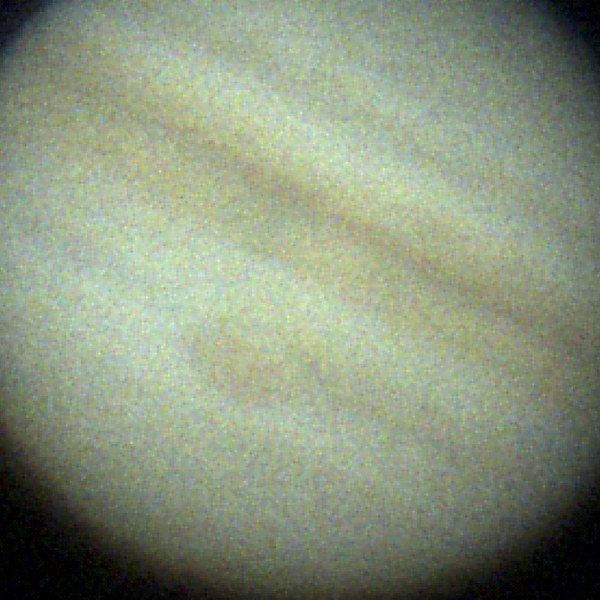
\includegraphics[width=0.8\linewidth]{figures/frame_best}
  \captionof{figure}{品質がいちばん高いフレーム}
\end{minipage}\hfill
\begin{minipage}[t]{0.47\linewidth}\centering
  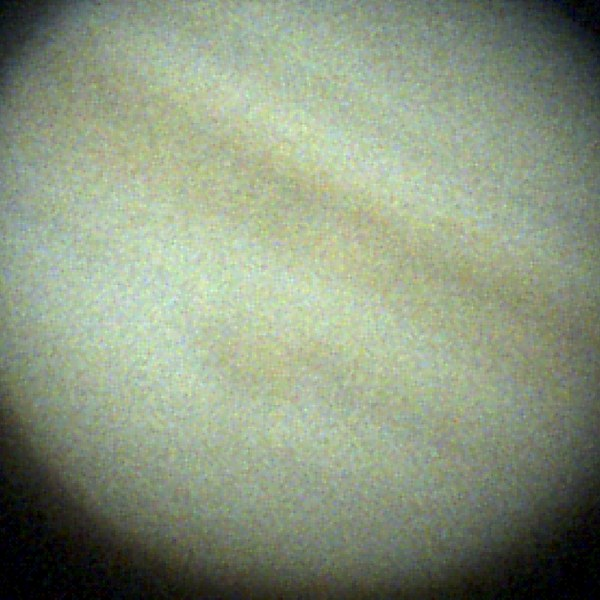
\includegraphics[width=0.8\linewidth]{figures/frame_worst}
  \captionof{figure}{品質がいちばん低いフレーム}
\end{minipage}

\medskip
1枚ずつではどちらもノイズが多く、差は分かりにくいかもしれません。拡大（\uil{200\%}）して縞模様の見え方を比べてみてください。
この「わずかな差」を数千枚ぶん積み重ねるのがスタックです。
% ------------------------------------------------------------------------------
\section{アライメント ——位置を合わせる}\label{sec:qs-align}

\begin{step}{3}{\ui{アライメント} を押す}
  \ui{アライメント} を押します（\key{shift}\key{⌘}\key{A} でも同じ）。次のことを自動で行います。
  \begin{enumerate}[label=(\alph*), itemsep=0pt, topsep=2pt]
    \item 品質の上位25\%のフレームを重ねて、\textbf{参照画像}（お手本）を作る
    \item 惑星の上に\textbf{位置合わせ領域}（四角います目）を自動で並べる
    \item 全フレームについて、ます目ごとに「お手本からどれだけずれているか」と「写りのよさ」を測る
  \end{enumerate}
  終わると「スタック」タブに切り替わって止まります。
\end{step}

\screen{qs_align}{アライメントが終わったところ}{%
  \mk[ne]{banner}{1}\mkd[inw]{preview}{2}\mk[s]{ref}{3}\mk[se]{apcount}{4}\mk[w]{tabs}{5}\mk[w]{aptop}{6}\mk[n]{stack}{7}}

\begin{marklist}
  \item 壊れたフレームや、追跡に失敗したフレーム（惑星が画面の外に出た、など）は自動で除外され、ここに枚数が出ます（この例では 30 枚）。\ui{詳細…} で一覧と理由を見られます。
  \item \textbf{参照画像}と、その上に並んだ\textbf{位置合わせ領域}（水色の四角）。模様のある所にだけ置かれ、背景の暗い宇宙には置かれません。
  \item 表示は自動で \uil{参照} に切り替わっています。
  \item 位置合わせ領域の数と大きさ（ここでは 109 個・48 画素）。
  \item 「スタック」タブに切り替わっています。
  \item 位置合わせ領域ごとに、写りのよい上位何\%のフレームを重ねるか（初期値 10\%）。
  \item \ui{スタック} が押せるようになりました。
\end{marklist}

\begin{center}
\begin{tikzpicture}
  \node[inner sep=0] (ap) {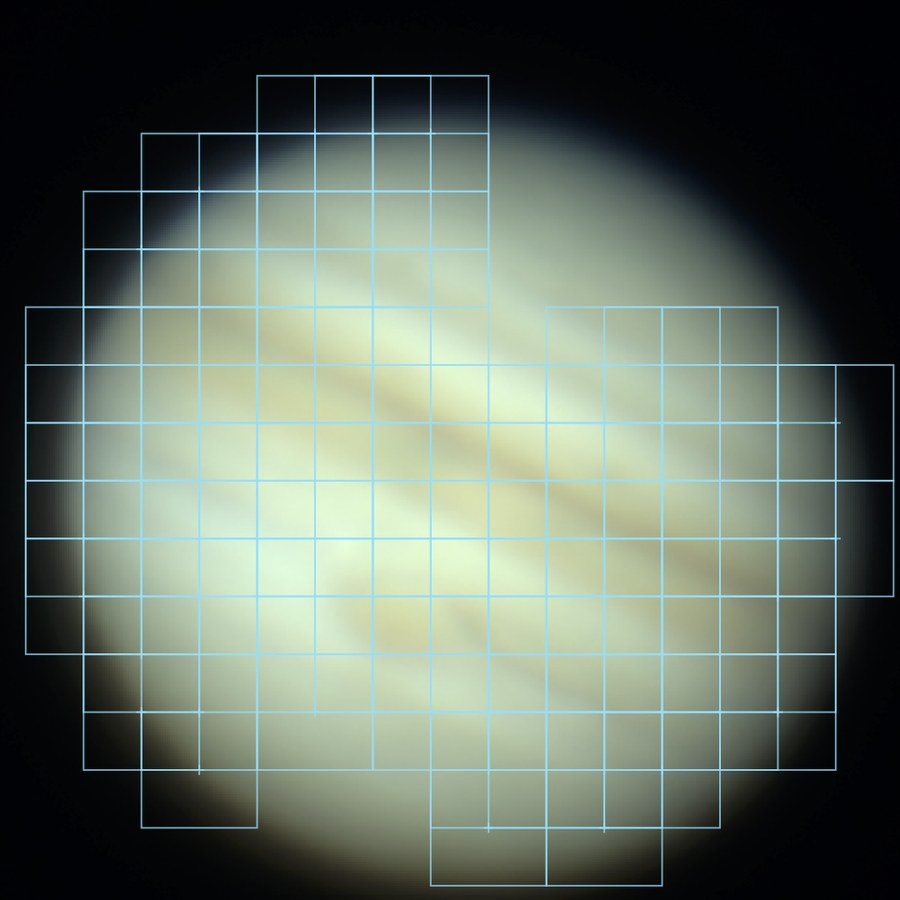
\includegraphics[width=0.5\linewidth]{figures/ap_zoom}};
  \node[lscallout, anchor=west, text width=0.4\linewidth] at ($(ap.east)+(0.5,0.9)$)
    {\small\textbf{なぜ小さな四角に分けるの？}\\[2pt]大気のゆらぎは、場所ごとにずれ方が違います。画像全体を1回で合わせると、
     ある場所は合っても別の場所はずれたままになります。四角ごとに合わせることで、画像全体がくっきりします。
     さらに四角ごとに写りのよいフレームを選ぶので、「このフレームは左上だけよく写っている」という瞬間も生かせます。};
\end{tikzpicture}
\captionof{figure}{参照画像と位置合わせ領域（拡大）}
\end{center}

% ------------------------------------------------------------------------------
\section{スタック ——重ね合わせる}\label{sec:qs-stack}

\begin{step}{4}{\ui{スタック} を押す}
  \ui{スタック} を押します（\key{⌘}\key{R}、またはこのボタンが青いときは \key{return}）。位置合わせ領域ごとに上位10\%のフレームを重ね、
  1枚の画像にまとめます。終わると表示が \uil{結果} に、タブが「仕上げ・出力」に切り替わります。
\end{step}

\screen{qs_stacked}{スタックが終わったところ}{%
  \mkd[inw]{preview}{1}\mk[s]{result}{2}\mk[w]{tabs}{3}\mkd[w]{wavelet}{4}\mk[n]{restack}{5}\mk[n]{export}{6}}

\begin{marklist}
  \item スタックの結果。1枚のフレームと比べて、ざらつきが大きく減っています。ただし、まだ少しぼんやりしています。
        これを次の「仕上げ」でくっきりさせます。
  \item 表示は \uil{結果} になっています。\uil{フレーム} や \uil{参照} に戻して見比べることもできます。
  \item 「仕上げ・出力」タブ。
  \item ウェーブレットなどの仕上げの設定。
  \item 採用率などを変えたら \ui{再スタック}。\textbf{品質評価とアライメントはやり直さない}ので、数秒で終わります。
  \item \ui{書き出し…} が押せるようになりました。
\end{marklist}

\begin{tip}[採用率を変えて試す]
  スタックタブの「位置合わせ領域ごとに採用するフレーム（\%）」を変えて \ui{再スタック} すると、すぐに結果を比べられます。
  上位の割合を減らすと、よい瞬間だけを使うのでシャープになりますが、重ねる枚数が減るのでノイズは増えます。
  目安は第\ref{sec:setting-aptop}節を見てください。
\end{tip}

% ------------------------------------------------------------------------------
\section{仕上げ ——細部を引き出す}\label{sec:qs-finish}

\begin{step}{5}{「仕上げ・出力」タブで調整する}
  仕上げは、スタックの結果を書き換えずに、見え方だけを調整します（何度でもやり直せます）。
  つまみを動かすと、プレビューがすぐに変わります。惑星なら、次の順に進めるのがおすすめです。
  \begin{enumerate}[label=(\alph*), itemsep=1pt, topsep=2pt]
    \item \textbf{RGB チャンネル合わせ}の \ui{自動で合わせる}：縁の赤・青のにじみを取ります。
    \item \textbf{ウェーブレット}：Layer 1〜3 の\uil{強調}を上げて細部を出し、\uil{ノイズ}でざらつきを抑えます。
    \item \textbf{色}の \ui{自動（灰色仮説）}：色かぶりを取ります。必要なら\uil{彩度}を少し上げます。
    \item \textbf{明るさ（レベル補正）}：黒と白の範囲を整えます。
  \end{enumerate}
\end{step}

この例では、次の値にしました（数値の決め方は第\ref{chap:finish}章）。

\begin{center}\small
\begin{tabular}{@{}lcccccc@{}}
\toprule
 & Layer 1 & Layer 2 & Layer 3 & Layer 4 & Layer 5 & Layer 6\\
\midrule
強調 & 12.00 & 7.00 & 3.00 & 1.50 & 1.00 & 1.00\\
ノイズ & 0.45 & 0.25 & 0.05 & 0.00 & 0.00 & 0.00\\
\bottomrule
\end{tabular}
\quad RGB 合わせ・色は \ui{自動}
\end{center}

\noindent
\begin{minipage}[t]{0.32\linewidth}\centering
  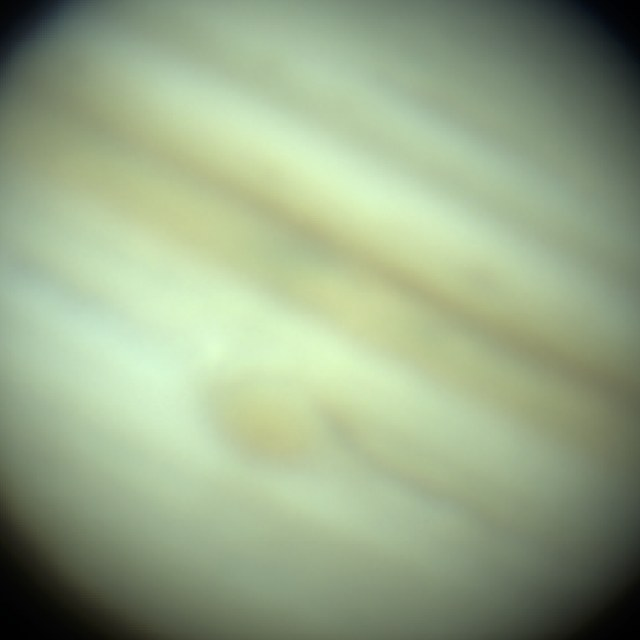
\includegraphics[width=\linewidth]{figures/before_stack}
  \captionof{figure}{スタックしただけ}
\end{minipage}\hfill
\begin{minipage}[t]{0.32\linewidth}\centering
  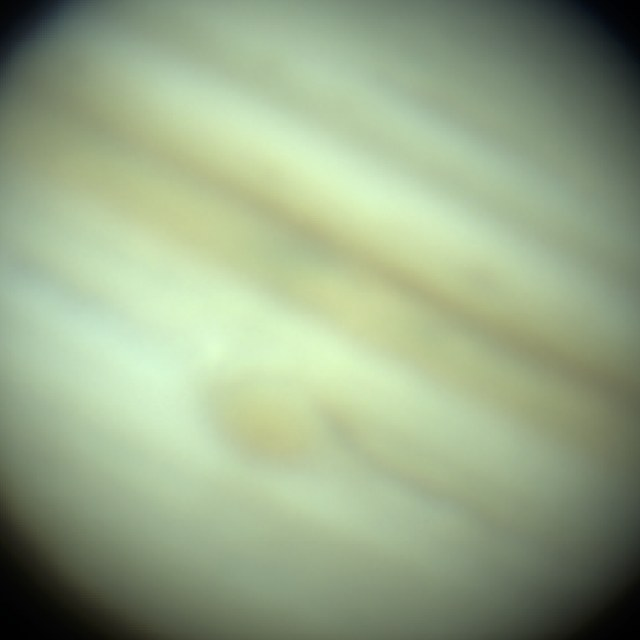
\includegraphics[width=\linewidth]{figures/after_nowave}
  \captionof{figure}{RGB 合わせと色だけ}
\end{minipage}\hfill
\begin{minipage}[t]{0.32\linewidth}\centering
  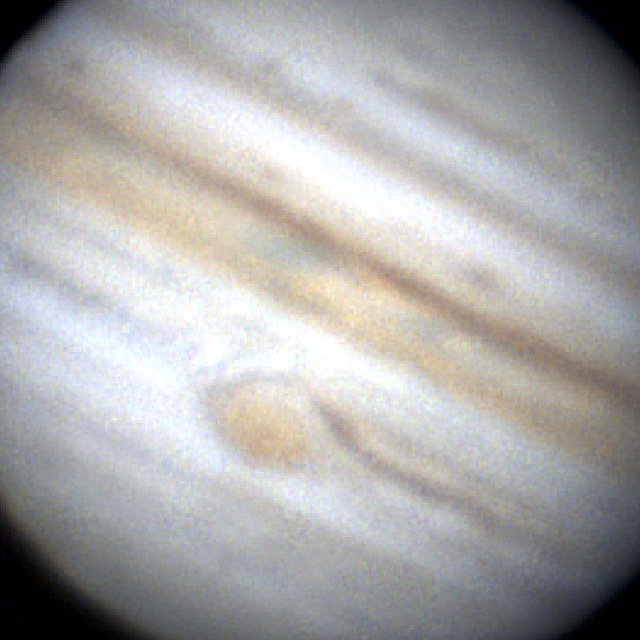
\includegraphics[width=\linewidth]{figures/after_finish}
  \captionof{figure}{ウェーブレットまで}
\end{minipage}

\medskip
ウェーブレットで、縞模様や大赤斑の細部がはっきり見えるようになりました。
強調しすぎるとノイズやふちの不自然な輪（リンギング）が目立つので、プレビューを拡大して確かめながら調整します。

\begin{tip}[効果あり・なしを見比べる]
  「仕上げ・出力」タブのいちばん上の \uil{仕上げ全体の効果をプレビュー} をオフにすると、スタックそのままの画像が出ます。
  ウェーブレット欄の \uil{ウェーブレットの効果をプレビュー} をオフにすると、ウェーブレットだけを外した画像が出ます。
  どちらも\textbf{表示の比較だけ}で、書き出すファイルには設定中の仕上げがすべて入ります。
\end{tip}

% ------------------------------------------------------------------------------
\section{書き出し ——ファイルに保存する}\label{sec:qs-export}

\begin{step}{6}{\ui{書き出し…} を押す}
  「仕上げ・出力」タブのいちばん下の「書き出し」欄で形式を選び、\ui{名前を付けて書き出し…}（または画面下の \ui{書き出し…}、\key{⌘}\key{S}）
  を押します。保存先を選ぶ画面が出るので、場所を決めて保存します。
\end{step}

\sidebyside[0.44]{qs_export}{%
  \mk[w]{format}{1}\mk[w]{name}{2}\mk[w]{object}{3}\mk[w]{meta}{4}\mk[w]{filename}{5}\mk[w]{save}{6}\mk[w]{multi}{7}}{%
  \begin{marklist}
    \item \textbf{形式}：ふつうは \uil{16bit TIFF}。PixInsight などで後処理を続けるなら \uil{32bit float FITS} が便利です。
    \item \textbf{ファイル名の付け方}：\uil{元の名前＋処理条件}、または WinJUPOS で使う \uil{WinJUPOS形式（撮影時刻を先頭に）}。
    \item \textbf{対象名}：「Jupiter」のように入れると、ファイル名と記録に入ります。
    \item 処理条件と撮影時刻をファイルの中に記録します。
    \item 付けられるファイル名の見本（例：\texttt{jupiter\_ap48\_10pct.tif}＝位置合わせ領域 48 画素・採用 10\%）。
    \item 保存します。
    \item 採用率を変えた結果をまとめて保存します（第\ref{sec:multiexport}節）。
  \end{marklist}}

\begin{point}[おつかれさまでした]
  これで一通りの処理ができました。同じファイルを次に開いたときは、保存されたサイドカーから解析結果を読み込むので、
  \ui{スタック} から始められます。次の章からは、各タブの設定をくわしく説明します。
\end{point}

\chapter{「品質評価」タブの設定}\label{chap:quality}

ここからは、右の設定パネルのタブごとに、設定の意味と数値の決め方を説明します。
各設定の枠の右上に、\textbf{既定値（初期値）}と\textbf{範囲・選択肢}を書いています。\textbf{\color{lsblue}目安}は、迷ったときの出発点です。

\begin{point}[まずは既定値で]
  既定値は、多くの惑星・月の動画でそのままうまくいくように選んであります。最初は変えずに処理し、結果を見てから1つずつ変えてください。
  一度に多くを変えると、何が効いたのか分からなくなります。
\end{point}

品質評価タブの設定は、\textbf{ファイルの読み方}と、\textbf{品質の測り方}を決めます。
ここを変えると、品質評価からやり直しになります。

% ------------------------------------------------------------------------------
\section{各フレームの品質評価}

\sidebyside[0.5]{insp_quality}{\mk[e]{metric}{1}\mk[e]{byteorder}{2}\mk[e]{depth}{3}}{%
  \begin{marklist}
    \item 品質指標
    \item バイトオーダー（SER のみ）
    \item ビット深度の解釈
  \end{marklist}
  ふつうは3つとも既定のままでかまいません。\badge{2}\,\badge{3} は、画像がおかしく見えるときにだけ変えます。}

\begin{setting}{\badge{1} 品質指標}{勾配エネルギー}{勾配エネルギー／周波数帯パワー比}
  フレームの「写りのよさ」を何で測るかを選びます。
  \begin{itemize}[itemsep=0pt, topsep=2pt]
    \item \uil{勾配エネルギー}：明るさの変化（ふち・模様）がどれだけくっきりしているかで測ります。軽くぼかしてから測るので、細かいノイズには反応しにくくなっています。
    \item \uil{周波数帯パワー比}：画像を周波数（模様の細かさ）に分け、中くらい〜細かい模様の強さの割合で測ります。
  \end{itemize}
  \meyasu{まずは \uil{勾配エネルギー}。品質グラフの順位が、自分の目で見た「よいフレーム」と合わないときに \uil{周波数帯パワー比} も試してください。}
\end{setting}

\begin{setting}{\badge{2} バイトオーダー（SERのみ）}{自動判定}{自動判定／little を使う／big を使う}
  16bit の SER ファイルで、2バイトの数値をどちらの順で読むかです。撮影ソフトによってはヘッダの記録が実際と逆のことがあり、
  \LS は中身を見て自動で判定します。
  \meyasu{画像が砂嵐のようにざらざらに壊れて見えるときだけ、\uil{little を使う}／\uil{big を使う} を切り替えてください。
  画面上部の警告の帯のボタンからも切り替えられます（第\ref{sec:byteorder}節）。}
\end{setting}

\begin{setting}{\badge{3} ビット深度の解釈}{ヘッダに従う}{ヘッダに従う／12bit として扱う／14bit として扱う}
  12bit や 14bit のカメラの画像が、16bit の入れ物に入っていることがあります。そのまま 16bit として読むと、画像がとても暗くなります。
  \meyasu{画像が極端に暗く、警告の帯に「12bitデータが16bitコンテナに入っている可能性があります」と出たら、\uil{12bit として扱う} を選びます。}
\end{setting}

% ------------------------------------------------------------------------------
\section{処理範囲}\label{sec:roi}

大きなセンサーで撮り、画面の一部にだけ対象が写っているときに、\textbf{その周りだけ}を処理する機能です。
処理が速くなり、メモリも少なくて済みます。

\sidebyside[0.5]{insp_roi}{\mk[e]{draw}{1}\mk[e]{label}{2}\mk[e]{clear}{3}}{%
  \begin{marklist}
    \item \uil{フレームの上で処理範囲を描く}：オンにして、プレビューの上でドラッグして四角を描きます。
    \item いまの範囲（大きさと位置）が出ます。
    \item \ui{全体に戻す}：範囲を消して、画像全体を処理します。
  \end{marklist}}

使い方と画面の例は第\ref{sec:roi-howto}節で説明します。
範囲を変えると、品質評価からやり直しになります。範囲はファイルごとの設定なので、プリセットには保存されません。

% ------------------------------------------------------------------------------
\section{入力の前処理（範囲・色・補正）}

\sidebyside[0.5]{insp_input}{\mk[e]{range}{1}\mk[e]{bayer}{2}\mk[e]{debayer}{3}\mk[e]{dark}{4}\mk[e]{flat}{5}\mk[e]{clearcal}{6}}{%
  \begin{marklist}
    \item 使うフレームの範囲
    \item 色の配列（Bayer）
    \item デバイヤーの方式
    \item ダーク
    \item フラット
    \item 補正をやめる
  \end{marklist}}

\begin{setting}{\badge{1} 使うフレームの範囲}{空欄（全体）}{1〜最後のフレーム番号}
  動画の一部だけを使います。左に最初、右に最後のフレーム番号を入れます。空欄なら最初から最後まで使います。
  \meyasu{途中で雲が通った、ピントを直した、など、品質グラフの\uil{時系列}で悪い区間がはっきり分かるときに、その区間を外します。
  惑星は自転するので、長すぎる動画（木星なら2〜3分を大きく超えるもの）は範囲を絞ると模様の流れを抑えられます。}
\end{setting}

\begin{setting}{\badge{2} 色の配列（Bayer）}{ヘッダに従う}{ヘッダに従う／モノクロとして扱う／RGGB／GRBG／GBRG／BGGR}
  カラーカメラのセンサーの色の並び方です。ふつうはファイルに記録されているので、自動で正しく読まれます。
  \meyasu{色がおかしい（全体が緑・紫になる、細かい格子模様が出る）ときは、ヘッダが間違っている可能性があります。
  4種類の並びを順に試し、自然な色になるものを選びます。モノクロのカメラなのに色付きで読まれてしまうときは \uil{モノクロとして扱う}。}
\end{setting}

\begin{setting}{\badge{3} デバイヤーの方式}{標準（bilinear）}{標準（bilinear）／高品質（Malvar-He-Cutler）}
  カラーの画素から3色をそろえる計算の方法です。
  \meyasu{\uil{高品質} のほうが細かい模様の色のにじみが少なく、少しシャープです。計算は少し重くなります。ふだんは \uil{標準} で十分です。}
\end{setting}

\begin{setting}{\badge{4}\,\badge{5} ダーク・フラット}{なし}{動画・静止画・静止画のフォルダ}
  \begin{itemize}[itemsep=0pt, topsep=2pt]
    \item \textbf{ダーク}：レンズにふたをして、本番と同じ露出・ゲイン・温度で撮った画像です。センサーの熱かぶりや、いつも明るい画素（ホットピクセル）を引き算で取り除きます。
    \item \textbf{フラット}：明るさが一様な面（薄曇りの空や、白い布ごしの光）を撮った画像です。周辺が暗くなる現象（周辺減光）や、センサーのホコリの影を割り算で補正します。
  \end{itemize}
  \ui{ダークを選ぶ…}\ui{フラットを選ぶ…} で、動画・静止画・静止画のフォルダを選びます。全フレームを平均して「マスター」を作り、デバイヤーの前の画素に掛けます。
  \meyasu{惑星の短い露出では、なくても大きな問題にならないことが多いです。月・太陽の広い視野で周辺減光やホコリの影が気になるときはフラットを、
  長めの露出や高いゲインでホットピクセルが目立つときはダークを使います。}
\end{setting}

\begin{setting}{\badge{6} 補正をやめる}{—}{—}
  選んだダーク・フラットを外します。
\end{setting}

% ------------------------------------------------------------------------------
\section{詳細設定（追跡失敗の判定）}

品質評価のときに、\textbf{使えないフレーム}（惑星が画面の外へ出た、雲で消えた、大きくぶれた、など）を自動で除外する基準です。

\sidebyside[0.5]{insp_qadv}{\mk[w]{outlier}{1}\mk[w]{similarity}{2}\mk[w]{maxshift}{3}}{%
  \begin{marklist}
    \item 外れ値判定の厳しさ（σ）
    \item 参照との類似度の下限
    \item 許容する位置ずれ（px）
  \end{marklist}
  除外したフレームは、アライメントのあとに警告の帯で枚数が出て、\ui{詳細…} で一覧と理由を見られます。}

\begin{setting}{\badge{1} 外れ値判定の厳しさ（σ）}{6.0}{正の数}
  お手本（参照）との似ている度合い（類似度）が、ほかのフレームと比べて飛び抜けて低いフレームを除外する基準です。全フレームの類似度の真ん中の値（中央値）から、ばらつきの何倍（σ、シグマ）離れたら除外するかを決めます。
  \meyasu{小さくするほど厳しく除外します。崩れたフレームが混ざって結果が乱れるときは 4〜5 に下げます。除外されすぎるときは 8〜10 に上げます。}
\end{setting}

\begin{setting}{\badge{2} 参照との類似度の下限}{0.5}{0〜1}
  お手本（参照）と比べた似ている度合い（1 が完全に同じ）がこの値より低いフレームを除外します。
  \meyasu{雲で薄くなったフレームなどを除きたいときは 0.6〜0.7 に上げます。ゆらぎが大きい日にフレームが除外されすぎるときは 0.3〜0.4 に下げます。}
\end{setting}

\begin{setting}{\badge{3} 許容する位置ずれ（px）}{空欄（自動：画像の短い辺の 1/4）}{画素数}
  お手本からこれ以上ずれたフレームを除外します。
  \meyasu{架台の追尾が悪く、惑星が画面の中で大きく動いてしまった動画で、フレームが除外されすぎるときは大きくします。}
\end{setting}

\chapter{「アライメント」タブの設定}\label{chap:align}

アライメントタブの設定は、\textbf{お手本（参照画像）の作り方}と、\textbf{位置合わせ領域の置き方・合わせ方}を決めます。
ここを変えたら \ui{再アライメント} を押します（品質評価はやり直しません）。

% ------------------------------------------------------------------------------
\section{アライメント（位置合わせ）}

\sidebyside[0.5]{insp_align}{%
  \mk[e]{method}{1}\mk[e]{mode}{2}\mk[e]{apsize}{3}\mk[e]{search}{4}\mk[e]{placement}{5}\mk[e]{ref}{6}\mk[e]{refine}{7}\mk[e]{report}{8}}{%
  \begin{marklist}
    \item 位置合わせ方法
    \item 対象モード
    \item 位置合わせ領域の大きさ
    \item 位置ずれの探索範囲
    \item 位置合わせ領域の配置
    \item 参照フレーム（品質上位 \%）
    \item 参照の反復精密化（2パス）
    \item \textbf{結果の内訳}：アライメントが終わると出ます。
  \end{marklist}
  \smallskip
  \badge{8} には、自動で判定した対象モードとお手本にしたフレームの番号、除外したフレームの内訳、
  位置合わせ領域の数と大きさ、うまく合わなかった所をどう扱ったかが出ます。結果が変なときの手がかりになります。}

\begin{setting}{\badge{1} 位置合わせ方法}{複数領域の局所位置合わせ（推奨）}{複数領域の局所位置合わせ／画像全体の位置合わせのみ（高速）}
  \begin{itemize}[itemsep=0pt, topsep=2pt]
    \item \uil{複数領域の局所位置合わせ（推奨）}：画像を位置合わせ領域に分け、領域ごとにずれを合わせ、領域ごとに写りのよいフレームを選びます。
          大気のゆらぎによる場所ごとのゆがみまで直せるので、いちばんシャープになります。
    \item \uil{画像全体の位置合わせのみ（高速）}：画像全体を1つとして平行移動だけで合わせます。速いですが、場所ごとのゆがみは残ります。
          このときは、参照に使う割合（オレンジの線）がそのままスタックの採用率になります。
  \end{itemize}
  \meyasu{ふだんは \uil{複数領域}。とにかく早く結果を見たいとき、ゆらぎがとても小さい日には \uil{画像全体のみ} も使えます。}
\end{setting}

\begin{setting}{\badge{2} 対象モード}{自動}{自動／惑星／月・太陽}
  全体の位置合わせのやり方を、対象に合わせて選びます。
  \begin{itemize}[itemsep=0pt, topsep=2pt]
    \item \uil{惑星}：暗い背景の中の明るい円盤として扱い、その重心で大まかに合わせてから精密に合わせます。惑星が画面の中を動いても追いかけられます。
    \item \uil{月・太陽}：画面いっぱいの模様として、画像全体の模様の一致で合わせます。
  \end{itemize}
  \meyasu{\uil{自動} のままで、画像から判定されます（判定結果は \badge{8} に出ます）。月の欠け際のように、暗い部分が大きい月面で
  \uil{惑星} と判定されてうまくいかないときは、\uil{月・太陽} を選び直してください。}
\end{setting}

\begin{setting}{\badge{3} 位置合わせ領域の大きさ}{自動}{自動／32／48／64／96／128／200 px}
  位置合わせ領域（四角）1つの一辺の画素数です。\uil{自動} では、対象の明るい部分の広がりから決めます（例：448 画素の木星では 48 画素、
  1024×768 の月面では 128 画素）。隣どうしの四角は半分ずつ重なるように並びます。
  \begin{itemize}[itemsep=0pt, topsep=2pt]
    \item \textbf{小さくする}と、細かい場所ごとのゆがみに追いつけますが、四角の中の模様が少なくなり、ノイズで合わせ間違えやすくなります。
    \item \textbf{大きくする}と、合わせ方は安定しますが、場所ごとのゆがみの補正は粗くなります。
  \end{itemize}
  \meyasu{まず \uil{自動}。ゆらぎが大きい日で、スタック結果の一部がぼやけるときは1段小さく、模様の少ない対象（金星・火星のうす模様）で
  結果がゆがむときは1段大きくします。惑星の円盤に数十〜百数十個並ぶくらいが目安です。}
\end{setting}

\begin{setting}{\badge{4} 位置ずれの探索範囲}{±16 px}{±8〜±32 px}
  位置合わせ領域ごとに、お手本からどこまでずれた所を探すかです。
  \meyasu{ゆらぎが大きく、像が大きく踊る日は ±24〜±32。小さい像やゆらぎの小さい日は ±8〜±12 にすると速く、合わせ間違いも減ります。
  結果の内訳の「一致度不足で補間」が多いときは、範囲を広げると改善することがあります。}
\end{setting}

\begin{setting}{\badge{5} 位置合わせ領域の配置}{自動配置}{自動配置に戻す／すべて消去}
  \ui{自動配置に戻す} で、手で足したり消したりした配置を自動の配置に戻します。\ui{すべて消去} で全部消し、自分で置き直せます（第\ref{sec:apedit}節）。
\end{setting}

\begin{setting}{\badge{6} 参照フレーム（品質上位 \%）}{25 \%}{5〜50 \%}
  品質の上位何\%のフレームを重ねてお手本を作るかです。品質グラフのオレンジの線と連動します。
  \meyasu{お手本はくっきりしていてノイズが少ないほど合わせやすくなります。フレームが数千枚あれば 10〜25\%、
  数百枚しかなければ 25〜50\% にして、お手本のノイズを減らします。}
\end{setting}

\begin{setting}{\badge{7} 参照の反復精密化（2パス）}{オン}{オン／オフ}
  一度位置を合わせて作った結果を新しいお手本にして、もう一度合わせ直します。お手本がよりシャープになり、位置合わせの精度が上がります。
  \meyasu{オンのまま。アライメントの時間を短くしたいときだけオフにします。}
\end{setting}

\begin{tip}[結果の内訳の読み方]
  \begin{itemize}[itemsep=0pt, topsep=2pt]
    \item \uil{除外：類似度不足 / 位置ずれ超過 / 外れ値}：品質評価タブの詳細設定（第\ref{chap:quality}章）の基準で除外した枚数です。
    \item \uil{一致度不足で補間}：模様がはっきりせず、うまく合わなかった位置合わせ領域の割合。その領域は周りの領域のずれから補って使います。
          惑星の縁や模様の少ない所では、ある程度出るのが普通です。
    \item \uil{近傍との差で制限}：隣の領域と比べて不自然に大きくずれた結果を抑えた割合。
    \item \uil{共通の位置ずれへ退避}：1枚のフレームの中で領域ごとのずれがばらばらで信用できないとき、そのフレームは全体に共通のずれだけで合わせます。
          木星の縞のように模様が一方向に並んだ対象では、この割合が高くなることがあります。
  \end{itemize}
\end{tip}

% ------------------------------------------------------------------------------
\section{詳細設定（位置合わせ領域）}

\sidebyside[0.5]{insp_aadv}{\mk[w]{minscore}{1}\mk[w]{gradient}{2}\mk[w]{level}{3}}{%
  \begin{marklist}
    \item 一致度の下限（下回ると補間）
    \item 配置する模様の強さ（比）
    \item 配置する明るさ（比）
  \end{marklist}}

\begin{setting}{\badge{1} 一致度の下限（下回ると補間）}{0.5}{0〜1}
  位置合わせ領域ごとの「お手本との一致度」（1 が完全に一致）がこの値より低いときは、その結果を使わず、周りの領域のずれから補います。
  \meyasu{合わせ間違いでスタック結果の一部が崩れるときは 0.6〜0.7 に上げます。補間が多すぎる（内訳の「一致度不足で補間」が大きい）ときは 0.3〜0.4 に下げます。}
\end{setting}

\begin{setting}{\badge{2}\,\badge{3} 配置する模様の強さ・明るさ（比）}{0.6・0.15}{0〜1 くらい}
  自動配置で、位置合わせ領域を置く場所の条件です。画像の中でいちばん強い模様・いちばん明るい所に対する割合で決めます。
  模様が弱すぎる所や暗すぎる所（背景の宇宙など）には置きません。
  \meyasu{月の欠け際の暗い所や、模様の乏しい所にも置きたいときは、模様の強さを 0.3〜0.4、明るさを 0.05〜0.1 に下げます。
  背景のノイズの上にまで置かれてしまうときは上げます。}
\end{setting}

% ------------------------------------------------------------------------------
\section{位置合わせ領域を手で置く}\label{sec:apedit}

自動の配置が気に入らないときは、手で足したり消したりできます。

\begin{enumerate}[itemsep=2pt]
  \item プレビューの下の \uil{配置を編集} をオンにします。
  \item プレビューを\textbf{クリック}すると、その場所に位置合わせ領域が1つ増えます。
  \item 領域をクリックして選び、\key{delete} を押すと消えます。
  \item 間違えたら \key{⌘}\key{Z} で取り消し、\key{shift}\key{⌘}\key{Z} でやり直しです。
  \item 配置を変えたら \ui{再アライメント} を押します。
\end{enumerate}

\begin{caution}
  手で置いた配置は、\ui{自動配置に戻す} を押すまで使われます。別のファイルを開いたときは自動の配置に戻ります。
\end{caution}

% ------------------------------------------------------------------------------
\section{品質で色分けする}\label{sec:heatmap}

プレビューの下の \ui{表示} メニューで \uil{品質で色分け} を選ぶと、位置合わせ領域の枠が、その場所の品質の平均で色分けされます。
青いほど品質が低く、緑・黄・赤になるほど高い場所です。「どこが最後までゆらぎに負けていたか」が分かります。

\screen[0.72\linewidth]{heatmap}{品質で色分けした位置合わせ領域}{\mk[ne]{legend}{1}}

\begin{marklist}
  \item 色の見本（左が品質が低い、右が高い）。
\end{marklist}

\chapter{「スタック」タブの設定}\label{chap:stack}

スタックタブの設定は、\textbf{どのフレームを・どう重ねるか}を決めます。
ここの設定の多くは、変えても \ui{再スタック} だけで済みます（品質評価・アライメントはやり直しません）。
いろいろ試して比べるのに向いた設定です。

% ------------------------------------------------------------------------------
\section{スタック（画像の合成）}

\sidebyside[0.5]{insp_stack}{%
  \mk[e]{selmode}{1}\mk[e]{aptop}{2}\mk[e]{normalize}{3}\mk[e]{method}{4}\mk[w]{sigma}{5}\mk[e]{lowmem}{6}\mk[e]{rawcfa}{7}}{%
  \begin{marklist}
    \item フレームの選択方式
    \item 位置合わせ領域ごとに採用するフレーム
    \item 輝度正規化
    \item 加算方式
    \item σクリップの閾値
    \item 低メモリモード
    \item Bayer のまま合成する
  \end{marklist}
  \smallskip
  \uil{これだけを変えた再スタックは解析をやり直しません} とあるとおり、\badge{1}\,\badge{2} を変えても \ui{再スタック} だけで結果を見られます。}

\begin{setting}{\badge{1} フレームの選択方式}{割合}{割合／枚数}
  \badge{2} を「上位何\%」で決めるか、「上位何枚」で決めるかを選びます。
  \meyasu{動画の長さがまちまちでも同じ感覚で使えるのは \uil{割合}。ノイズの量をそろえたいとき（毎回200枚重ねる、など）は \uil{枚数}。}
\end{setting}

\begin{setting}{\badge{2} 位置合わせ領域ごとに採用するフレーム}{10 \%}{1〜100 \%（枚数のときは 1〜全フレーム数）}\label{sec:setting-aptop}
  位置合わせ領域ごとに、その場所の写りがよい順に何\%（何枚）を重ねるかです。\textbf{スタックの仕上がりをいちばん大きく左右する設定}です。
  \begin{center}
  \begin{tikzpicture}[font=\sffamily\scriptsize]
    \shade[left color=lsblue!70, right color=lsorange!80] (0,0) rectangle (9,0.35);
    \node[anchor=north west, align=left] at (0,-0.05) {少なくする（例 3〜5\%）\\よい瞬間だけ → シャープ\\重ねる枚数が減る → ざらつく};
    \node[anchor=north east, align=right] at (9,-0.05) {多くする（例 30〜50\%）\\悪い瞬間も混ざる → ぼやける\\枚数が増える → なめらか};
    \draw[white, line width=1.2pt] (1.8,0) -- (1.8,0.35); \node[above] at (1.8,0.35) {10\%（既定）};
  \end{tikzpicture}
  \end{center}
  \meyasu{重ねる枚数が\textbf{位置合わせ領域あたり 100〜500 枚}くらいになるのが1つの目安です（枚数＝使うフレーム数×割合。例：4617 フレームの 10\%＝約 460 枚）。
  \begin{itemize}[itemsep=0pt, topsep=1pt]
    \item 数千フレームの惑星動画：5〜15\%
    \item 数百フレームしかない、または暗くノイズが多い：20〜40\%
    \item ゆらぎがとても小さい日：多めにしてもシャープさが落ちにくい
  \end{itemize}
  迷ったら、「書き出し」欄の \uil{複数の採用率で書き出す} に \texttt{5, 10, 25} のように入れてまとめて作り、見比べるのが確実です（第\ref{sec:multiexport}節）。}
\end{setting}

\begin{setting}{\badge{3} 輝度正規化}{オン}{オン／オフ}
  薄い雲や空の透明度の変化で、フレームごとに明るさが変わることがあります。重ねる前に、各フレームの明るさをお手本にそろえます。
  \meyasu{オンのまま。明るさが本当に変わる現象を記録したいとき（ふつうは無い）だけオフにします。}
\end{setting}

\begin{setting}{\badge{4} 加算方式}{単純平均}{単純平均／品質重み付き平均／σクリップ}
  \begin{itemize}[itemsep=0pt, topsep=2pt]
    \item \uil{単純平均}：選んだフレームを同じ重みで平均します。
    \item \uil{品質重み付き平均}：品質が高いフレームほど重く数えます。シャープさを少し優先します。
    \item \uil{σクリップ}：画素ごとに、ほかのフレームと飛び抜けて違う値（人工衛星・飛行機の光跡、宇宙線、ホットピクセルなど）を除いて平均します。
  \end{itemize}
  \meyasu{ふだんは \uil{単純平均}。光跡や白い点が写り込んだときは \uil{σクリップ}（重ねる枚数が 20 枚以上あるときに効きます）。}
\end{setting}

\begin{setting}{\badge{5} σクリップの閾値（σ）}{2.0}{正の数（σクリップのときだけ使える）}
  平均からばらつきの何倍（σ）離れた値を除くかです。
  \meyasu{小さいほど多くの値を除きます。2.0〜3.0。光跡が消えきらないときは下げ、ノイズが増えたように見えるときは上げます。}
\end{setting}

\begin{setting}{\badge{6} 低メモリモード（2GB上限）}{オフ}{オン／オフ}
  スタック中に使うメモリをおよそ 2GB までに抑えます。結果は同じで、少し時間がかかることがあります。
  \meyasu{メモリの少ない Mac（4〜8GB）で、大きな画像やドリズル拡大のときに、ほかのアプリが重くなるならオンにします。}
\end{setting}

\begin{setting}{\badge{7} Bayer のまま合成する（デバイヤーしない）}{オフ}{オン／オフ}
  カラーカメラの画像を、色をそろえる前（Bayer 配列のまま）で重ね、そのまま書き出します。
  \meyasu{PixInsight など、ほかのソフトで後から色をそろえたい人向けです。ふだんはオフ。切り替えると品質評価からやり直しになります。}
\end{setting}

% ------------------------------------------------------------------------------
\section{ドリズル拡大}\label{sec:drizzle}

ドリズルは、フレームごとの細かな位置のずれを利用して、元の画素より細かい画素で画像を作り直す拡大の方法です。
\textbf{像が画素に対して粗く写っている（アンダーサンプリング）ときだけ}、解像度が上がります。
焦点距離が十分に長く、すでに細かく写っているときに倍率を上げても、ファイルが大きくなり処理が遅くなるだけです。

\sidebyside[0.5]{insp_drizzle}{\mk[e]{scale}{1}\mk[e]{pixfrac}{2}\mk[e]{diagnose}{3}\mkd[w]{result}{4}}{%
  \begin{marklist}
    \item 倍率
    \item 投影する画素の幅（pixfrac）
    \item \ui{ドリズルを診断}
    \item 診断の結果
  \end{marklist}
  \smallskip
  倍率を 1× 以外にすると、倍率の下に出力の大きさと作業に使うメモリの目安が出ます。}

\begin{setting}{\badge{1} 倍率}{1×（使わない）}{1×／1.5×／2×／3×}
  出力の画像を何倍の大きさで作るかです。変えたら \ui{再スタック}。
  \meyasu{まず \badge{3} の診断を押して、勧められた倍率にします。}
\end{setting}

\begin{setting}{\badge{2} 投影する画素の幅（pixfrac）}{0.90}{0.5〜1.0}
  1つの画素を、元の大きさの何割に縮めて新しい画素へ配るかです。小さいほどシャープになりますが、隙間ができてノイズやむらが出やすくなります。
  \meyasu{0.7〜0.9。重ねる枚数が多いほど小さくできます。まだらな模様が出たら大きくします。}
\end{setting}

\subsection*{\badge{3} ドリズルを診断}

アライメントのあとに \ui{ドリズルを診断} を押すと、スタックせずに数秒で「ドリズルが効きそうか・何倍まで効きそうか」の目安を出します。
次の3つを調べ、いちばん厳しいものを答えにします。

\begin{center}\small
\begin{tabularx}{0.95\linewidth}{@{}>{\sffamily\bfseries}l X@{}}
\toprule
像の細かさ & 画素で表せる最も細かい模様（ナイキスト周波数）を超えて、細部が写っているか。超えていれば、画素が粗すぎる＝ドリズルの出番です。\\
位置のばらつき & フレームごとの位置のずれが、1画素より細かい単位でばらけているか。ばらけていないと、細かい画素の隙間を埋められません。\\
採用枚数 & 位置合わせ領域あたりの枚数が足りるか。拡大すると1枚の寄与が細かい画素に分かれ、ノイズが増えます。\\
\bottomrule
\end{tabularx}
\end{center}

結果には、結論（\uil{効きそうです。目安は 2× までです。}または\uil{効果は小さそうです。等倍（1×）のままをおすすめします。}）と、
3つの理由が出ます。いちばん厳しかったものに\uil{（いちばんの制約）}と付きます。
効きそうなときは \ui{2× にする} のようなボタンが出て、押すと倍率を合わせます。
採用率を変えたり、アライメントをやり直したりすると、結果は消えます（もう一度押してください）。

\begin{caution}[診断は「ざっくりの目安」です]
  1枚の画像から見積もるので、正確な判定ではありません。確かめるには、倍率を変えてスタックし、拡大して見比べてください。
  背景の空が写っていない月面・太陽の全面では、控えめ（小さめ）に見積もります。
  上の画面の例では、木星の像はナイキストをわずかに超えるだけ（1.3倍）なので、1× を勧めています。
\end{caution}

\chapter{「仕上げ・出力」タブの設定}\label{chap:finish}

仕上げは、スタックの結果そのものは書き換えずに、見え方を調整する工程です。つまみを動かすと、プレビューがすぐに変わります。
何度動かしても元の画質は落ちないので、気軽に試してください。
仕上げは、\textbf{RGB チャンネル合わせ → ウェーブレット → 色 → 明るさ → 向き}の順に掛かります（順番は変わりません）。

% ------------------------------------------------------------------------------
\section{プレビューの比較}

\sidebyside[0.5]{insp_compare}{\mk[e]{all}{1}}{%
  \begin{marklist}
    \item \uil{仕上げ全体の効果をプレビュー}：オフにすると、仕上げを掛ける前のスタックの結果を表示します。
  \end{marklist}
  オン・オフは画面で見比べるためだけのもので、書き出すファイルには設定中の仕上げがすべて入ります。}

% ------------------------------------------------------------------------------
\section{RGB チャンネル合わせ（大気分散）}

低い空の惑星は、大気がプリズムのように働いて、赤い像と青い像が少しずれます（大気分散）。惑星の上下の縁に赤や青のにじみが出るのはこのためです。
赤（R）と青（B）の像を緑（G）に重ねて取り除きます。

\sidebyside[0.5]{insp_channel}{\mk[e]{fields}{1}\mk[e]{auto}{2}\mk[e]{reset}{3}}{%
  \begin{marklist}
    \item R・B をずらす量（画素、小数も可）。x は横、y は縦です。
    \item \ui{自動で合わせる}：画像から自動でずれを測って入れます。
    \item \ui{戻す}：0 に戻します。
  \end{marklist}
  \meyasu{まず \ui{自動で合わせる}。縁のにじみが残るときは、数値を 0.1 ずつ変えて調整します。モノクロの画像では使えません。}}

% ------------------------------------------------------------------------------
\section{ウェーブレット仕上げ}\label{sec:wavelet}

ぼんやりしたスタックの結果から、細部を引き出すための中心的な道具です。
画像を\textbf{模様の細かさごとに6つの層（レイヤー）}に分け、層ごとに強めたり、ざらつきを抑えたりします。

\begin{center}
\begin{tikzpicture}[font=\sffamily\scriptsize]
  \foreach \i/\n/\px in {0/1/2,1/2/4,2/3/8,3/4/16,4/5/32,5/6/64} {
    \begin{scope}[shift={(\i*2.25,0)}]
      \fill[black!85] (0,0) rectangle (1.8,1.8);
      \pgfmathsetmacro{\f}{2.6/(\n)}
      \begin{scope}
        \clip (0,0) rectangle (1.8,1.8);
        \foreach \k in {0,...,14} {
          \pgfmathsetmacro{\yy}{\k*0.14*(\n)}
          \draw[white, opacity=0.8, line width={0.9pt*\n*0.55}] (0,\yy) sin (0.9,{\yy+0.05*\n}) cos (1.8,\yy);
        }
      \end{scope}
      \node[below] at (0.9,0) {Layer \n（約\px px）};
    \end{scope}
  }
  \draw[-{Stealth}, line width=1pt] (0,-0.75) -- node[below]{細かい模様（ノイズもここに多い）\hspace{12em}大きな模様（明るさのむら）} (13.05,-0.75);
\end{tikzpicture}
\captionof{figure}{ウェーブレットの層のイメージ（層が上がるほど大きな模様）}
\end{center}

\sidebyside[0.5]{insp_wavelet}{%
  \mk[e]{preview}{1}\mk[w]{layer1}{2}\mk[w]{sharpen1}{3}\mk[w]{denoise1}{4}\mk[n]{reset1}{5}\mk[e]{linked}{6}\mk[w]{dering}{7}\mk[e]{resetall}{8}}{%
  \begin{marklist}
    \item \uil{ウェーブレットの効果をプレビュー}：オフにすると、ウェーブレット（と輪抑制）だけを外した画像を表示します（比較用）。
    \item 1つの層の設定。見出しの\uil{約2 px}は、その層が受け持つ模様の大きさです。
    \item \textbf{強調}：その層の模様を何倍にするか。\textbf{1.00 が変化なし}、2.00 で2倍。
    \item \textbf{ノイズ}：その層の小さな揺れ（ノイズ）をどれだけ消すか。0 で何もしない、大きいほど強く消します。
    \item \ui{初期値に戻す}：この層を強調 1.00・ノイズ 0.00 に戻します。
    \item \uil{レイヤーを連動}：オンにすると、いまの層ごとの配分を保ったまま、下の\uil{強さ}で全体の効き具合だけを変えられます。
    \item \textbf{輪抑制}：強調すると、明るい縁（惑星のふち）の外側に暗い輪ができることがあります。これを抑えます。
    \item \ui{すべてリセット}：全部の層を初期値に戻します。
  \end{marklist}
  \smallskip
  各行の \ui{－}\ui{＋} で少しずつ変えられ（押し続けると連続）、右の数値欄には直接数字を打てます。}

\begin{setting}{強調（Layer 1〜6）}{1.00（変化なし）}{0〜20}
  \meyasu{\textbf{細かい層から順に}上げていきます。惑星の例：
  \begin{center}\small
  \begin{tabular}{@{}lcccccc@{}}
  \toprule
   & Layer 1 & Layer 2 & Layer 3 & Layer 4 & Layer 5 & Layer 6\\
  \midrule
  控えめ & 4〜6 & 2〜3 & 1.3〜1.5 & 1.0 & 1.0 & 1.0\\
  しっかり & 8〜15 & 5〜8 & 2〜3 & 1.2〜1.5 & 1.0 & 1.0\\
  \bottomrule
  \end{tabular}
  \end{center}
  8 を超えるあたりから、細部と一緒にノイズや縁の輪も強くなります。\uil{100\%} や \uil{200\%} に拡大して確かめながら決めてください。
  月面の広い写野では、Layer 1〜2 を控えめに、Layer 3〜4 を少し上げると自然に見えます。}
\end{setting}

\begin{setting}{ノイズ（Layer 1〜6）}{0.00}{0〜1}
  \meyasu{強調を上げてざらつきが目立ってきたら、同じ層（特に Layer 1）のノイズを上げます。Layer 1 で 0.2〜0.5、Layer 2 で 0.1〜0.3。
  上げすぎると細部まで消えて、のっぺりします。}
\end{setting}

\begin{setting}{輪抑制（デリンギング）}{0.00}{0〜1}
  \meyasu{惑星の縁の外に黒い輪が見えたら 0.2〜0.5。上げすぎると縁の近くの細部が弱まります。}
\end{setting}

\begin{setting}{レイヤーを連動の強さ}{1.00}{0〜2.5}
  \meyasu{配分を決めたあと、「全体をもう少し弱く」したいときに 0.7〜0.9 などにします。}
\end{setting}

% ------------------------------------------------------------------------------
\section{色（ホワイトバランス・彩度）}

\sidebyside[0.5]{insp_color}{\mk[e]{gains}{1}\mk[e]{saturation}{2}\mk[e]{auto}{3}}{%
  \begin{marklist}
    \item R・G・B の倍率（0.5〜2.0、既定 1.0）。赤が強すぎれば R を下げる、のように使います。
    \item \textbf{彩度}（0〜2、既定 1.0）。0 で白黒、大きいほど色が濃くなります。
    \item \ui{自動（灰色仮説）}：画像全体の平均が灰色になるように R・B の倍率を決めます。\ui{戻す} で 1.0 に戻します。
  \end{marklist}
  \meyasu{まず \ui{自動（灰色仮説）}。そのあと好みで R・B を微調整し、彩度は 1.1〜1.4 くらいまで。
  カメラの RAW は緑がかって読まれるので、必ず \ui{自動} を押してください。}}

% ------------------------------------------------------------------------------
\section{明るさ（レベル補正）}\label{sec:levels}

Photoshop のレベル補正と同じ仕組みで、黒・中間・白の3つの三角を動かして明るさを決めます。

\sidebyside[0.5]{levels}{\mk[e]{channel}{1}\mkd[inw]{histogram}{2}\mkn[s]{black}{3}\mkn[s]{mid}{4}\mkn[s]{white}{5}\mk[e]{fields}{6}\mk[e]{auto}{7}
  \drag{($(white)+(0,-0.075)$)}{($(white)+(-0.15,-0.075)$)}}{%
  \begin{marklist}
    \item \textbf{チャンネル}：\uil{RGB}（全体）か、\uil{R}\uil{G}\uil{B} の1色ずつかを選びます。
    \item \textbf{ヒストグラム}：画像の中で、どの明るさの画素がどれだけあるかのグラフ。左が暗い、右が明るい画素です。
    \item \textbf{黒の三角}：これより暗い所を真っ黒にします。
    \item \textbf{中間の三角}：中間の明るさ。左へ動かすと全体が明るく、右へ動かすと暗くなります（数値はガンマ、1.00 が変化なし）。
    \item \textbf{白の三角}：これより明るい所を真っ白にします。矢印のように左へ動かすと、画像が明るく、コントラストが強くなります。
    \item 三角の位置の数値（黒 0〜255・中間のガンマ・白 0〜255）。直接打ち込むこともできます。
    \item \ui{自動}：明るさの分布から黒と白を自動で決めます。\ui{初期値に戻す} ですべて戻します。
  \end{marklist}}

\meyasu{惑星なら、黒は背景の山（ヒストグラムの左端の高い山）のすぐ右、白は惑星のいちばん明るい所がぎりぎり白くならない所。
中間は 0.9〜1.3。白を左に寄せすぎると明るい所が白く飛んで、模様が消えます。}

\begin{caution}[画面が明るく見える設定について]
  プレビューの \ui{表示} メニューの \uil{表示を明るくする} がオンの間は、暗い画像でも画面の上では見やすく引き伸ばしています。
  書き出すファイルと同じ明るさで見たいときは、これをオフにしてください。
\end{caution}

% ------------------------------------------------------------------------------
\section{向き・切り抜き}\label{sec:crop}

\sidebyside[0.5]{insp_geometry}{\mk[e]{rotate}{1}\mk[e]{flip}{2}\mk[e]{cropmode}{3}\mk[e]{cropbuttons}{4}}{%
  \begin{marklist}
    \item \ui{\rotl{} 左へ90°}\ui{右へ90° \rotr{}}：画像を90度ずつ回します。
    \item \uil{左右反転}\uil{上下反転}：鏡に映したように裏返します（望遠鏡の種類によって像が裏返っているとき）。
    \item \uil{プレビューで切り抜く枠を描く}：オンにすると、プレビューの上で切り抜く範囲を描けます。
    \item \ui{切り抜く}\ui{枠を消す}\ui{元に戻す}。
  \end{marklist}}

\screen{cropbox}{切り抜く枠を描いたところ}{%
  \mk[nw]{box}{1}\drag{($(box-se)+(0.03,-0.03)$)}{($(box-se)+(-0.02,0.02)$)}\mk[w]{cropmode}{2}\mk[s]{apply}{3}\mk[s]{clearbox}{4}\mk[s]{undo}{5}\mk[w]{rotate}{6}}

\begin{marklist}
  \item \textbf{切り抜く枠}（黄色の点線）。枠の外は暗く表示されます。
        \begin{itemize}[itemsep=0pt, topsep=1pt]
          \item 枠の外でドラッグ：新しく枠を描く
          \item 枠の内側でドラッグ：枠を動かす
          \item 辺や角（小さな四角の印）をドラッグ：大きさを変える（矢印）
        \end{itemize}
  \item 枠を描くモードのオン・オフ。
  \item \ui{切り抜く}：その場で画像が小さくなります。以降の仕上げも軽くなります。
  \item \ui{枠を消す}：枠だけを消します（画像はそのまま）。
  \item \ui{元に戻す}：切り抜く前の画像に戻します。
  \item 回転や反転をしたあとでも、見えている向きのまま枠を描けます。
\end{marklist}

\begin{tip}
  惑星の周りの黒い背景を少し残して切り抜くと、ファイルが小さくなり、SNS などに載せたときも見やすくなります。
  切り抜きはプリセットには保存されません。
\end{tip}

% ------------------------------------------------------------------------------
\section{書き出し}\label{sec:export}

\sidebyside[0.5]{insp_export}{\mk[e]{format}{1}\mk[e]{name}{2}\mk[w]{object}{3}\mk[e]{meta}{4}\mk[e]{save}{5}\mk[e]{multi}{6}}{%
  \begin{marklist}
    \item 形式
    \item ファイル名の付け方
    \item 対象名
    \item 処理条件と撮影時刻を記録する
    \item \ui{名前を付けて書き出し…}
    \item 複数の採用率で書き出す
  \end{marklist}}

\begin{setting}{\badge{1} 形式}{16bit TIFF}{16bit TIFF／32bit float TIFF／32bit float FITS（PixInsight向け）／16bit PNG}
  \begin{itemize}[itemsep=0pt, topsep=2pt]
    \item \uil{16bit TIFF}：多くの画像ソフトで開けます。ふつうはこれ。
    \item \uil{32bit float TIFF}・\uil{32bit float FITS}：明るさを小数のまま保存します。PixInsight・Siril などで、さらに処理を続けるとき向けです。
    \item \uil{16bit PNG}：ウェブに載せたり、手軽に見たりするとき向けです。
  \end{itemize}
\end{setting}

\begin{setting}{\badge{2} ファイル名の付け方}{元の名前＋処理条件}{元の名前＋処理条件／WinJUPOS形式（撮影時刻を先頭に）}
  \begin{itemize}[itemsep=0pt, topsep=2pt]
    \item \uil{元の名前＋処理条件}：例 \texttt{jupiter\_ap48\_10pct.tif}（位置合わせ領域 48 画素・採用 10\%）。ドリズルを使うと \texttt{\_x2} のように倍率も付きます。
    \item \uil{WinJUPOS形式}：例 \texttt{2026-08-09-1432\_5-Jupiter.tif}。撮影時刻の中央を先頭に付けます。木星・火星の自転を測るソフト WinJUPOS で使うとき向け。
          撮影時刻の記録が無いファイルでは、元の名前の方式になります。
  \end{itemize}
\end{setting}

\begin{setting}{\badge{3} 対象名（ファイル・メタデータ用）}{空欄}{文字}
  \texttt{Jupiter} のように入れると、ファイル名（元の名前の方式では元の名前の後ろ、WinJUPOS形式では時刻の後ろ）と、ファイルに記録する情報に入ります。WinJUPOS形式で空欄のときは、元の名前を使います。
\end{setting}

\begin{setting}{\badge{4} 処理条件と撮影時刻をファイルに記録する}{オン}{オン／オフ}
  使った設定（採用率・位置合わせ領域の大きさなど）と撮影時刻を、画像ファイルの中に書き込みます。あとで「どう処理したか」を確かめられます。
\end{setting}

\subsection*{\badge{6} 複数の採用率で書き出す}\label{sec:multiexport}

採用率を変えた結果を、一度にまとめて作って保存します。欄に \texttt{5, 10, 25} のようにカンマで区切って入れ、\ui{まとめて書き出し…} を押して保存先のフォルダを選びます。
スタックタブの選択方式が\uil{枚数}のときは、枚数として読みます（例 \texttt{100, 200, 400}）。

アライメントの結果を使い回してスタックだけをやり直し、\textbf{いまの仕上げ（切り抜きも含む）}を掛けて保存します。同じ名前のファイルがあっても上書きせず、番号を付けます。
どの採用率がよいか迷ったときに、並べて比べるのに便利です。

\chapter{いろいろな素材と便利な機能}\label{chap:sources}

% ------------------------------------------------------------------------------
\section{月・太陽を処理する}\label{sec:moon}

月面や太陽面は、画面いっぱいに模様が広がっています。処理の手順は惑星と同じで、多くの場合は既定値のままで大丈夫です。

\screen[0.78\linewidth]{moon_ap}{月面の参照画像と位置合わせ領域（1024×768、自動で 128 画素・124 個）}{}

\begin{itemize}[itemsep=2pt]
  \item \textbf{対象モード}は\uil{自動}で\uil{月・太陽}と判定されます。うまくいかないときはアライメントタブで\uil{月・太陽}を選びます。
  \item 位置合わせ領域は、画面の明るい所いっぱいに並びます。上の例では欠け際の暗い所には置かれていません。
        暗い所にも置きたいときは、詳細設定の\uil{配置する明るさ}を下げます（第\ref{chap:align}章）。
  \item 画面が大きい（例：1920×1200 以上）と時間がかかります。対象が画面の一部だけなら\textbf{処理範囲}（第\ref{sec:roi-howto}節）を使うと速くなります。
  \item ウェーブレットは、Layer 1〜2 を控えめ（2〜5 くらい）、Layer 3〜4 を少し上げると自然な仕上がりになりやすいです。
  \item 太陽の Hα など 16bit のモノクロ SER では、画面上部に「ヘッダと異なるバイトオーダーで読んでいます」と灰色で出ることがあります。
        画像が正常に見えていれば問題ありません（第\ref{sec:byteorder}節）。
\end{itemize}

% ------------------------------------------------------------------------------
\section{カメラの RAW・静止画を処理する}\label{sec:raw}

一眼レフ・ミラーレスで連写した RAW（CR2・CR3・NEF・ARW・RAF など）や、TIFF・PNG・JPEG・FITS の連番も扱えます。

\begin{enumerate}[itemsep=2pt]
  \item 画像を1つのフォルダにまとめ、\textbf{フォルダごと}入力キューへドロップします（複数の画像を選んでドロップしてもかまいません）。
        名前の順に並べた1本の「連番」として追加されます。
  \item あとは動画と同じく \ui{品質評価}\ui{アライメント}\ui{スタック} と進めます。
  \item RAW は、カメラの色の調整（ホワイトバランス・色の変換・明るさの曲線）を掛けない\textbf{そのままの明るさ（リニア）}で読みます。
        そのため、スタックの結果は\textbf{緑がかって暗く}見えます。仕上げの \ui{自動（灰色仮説）} で色を、レベル補正で明るさを整えてください。
\end{enumerate}

\begin{tip}[写真の枚数が少ないとき]
  連写が数枚〜数十枚しかないときは、スタックタブの採用率を大きく（30〜100\%）、アライメントタブの参照フレームも大きく（50\%）すると、
  ノイズの少ない結果になります。
\end{tip}

% ------------------------------------------------------------------------------
\section{処理範囲を使う}\label{sec:roi-howto}

大きなセンサー（例：6240×4160 画素）で撮り、月や惑星が画面の中央に小さく写っているだけなら、\textbf{処理範囲}を決めてその周りだけを処理すると、
何倍も速くなり、メモリも少なくて済みます。

\screen{cr2_roi}{カメラの RAW（8枚）で処理範囲を決めたところ}{%
  \mk{queuerow}{1}\mkd[nw]{roibox}{2}\mk[w]{draw}{3}\mk[w]{label}{4}\mk[w]{clear}{5}\mk[w]{status}{6}
  \drag{($(roibox-nw)+(0.015,-0.03)$)}{($(roibox-se)+(-0.015,0.03)$)}}

\begin{marklist}
  \item フォルダを追加すると、\uil{cr2（静止画連番）・8フレーム・6240×4160} のように1本の連番として並びます。
  \item \textbf{処理範囲}（黄色の点線）。品質評価タブの \uil{フレームの上で処理範囲を描く} をオンにし、プレビューの上でドラッグして描きます。
        枠の外でドラッグすると描き直し、内側で移動、辺や角で大きさを変えられます。
  \item 範囲を描くモードのオン・オフ。
  \item 決まった範囲（例：3120×2080 画素、左上が x 1560・y 1040）。
  \item \ui{全体に戻す}：範囲を消して全体を処理します。
  \item 範囲を変えると、品質評価からやり直しになります。
\end{marklist}

\begin{caution}[対象が範囲からはみ出さないように]
  撮影中、対象は少しずつ動きます。\textbf{余白を取って}囲み、フレームのスライダーを最後まで送って、対象が範囲に収まり続けているか確かめてください。
  品質評価・アライメントのあとに、はみ出すフレームがあればその数を知らせます。
\end{caution}

% ------------------------------------------------------------------------------
\section{MOV・MP4 の動画を処理する}\label{sec:movie}

スマートフォンやデジタルカメラの MOV・MP4・M4V（H.264・HEVC・ProRes など）も開けます。
HEVC（H.265）の動画は、macOS 10.13 以降でだけ読めます（10.12 には macOS 側に HEVC の読み込み機能がありません）。

\screen{mp4_banner}{MOV・MP4 を開いたときの注意の帯}{\mk[inw]{banner}{1}}

\begin{marklist}
  \item MOV・MP4 は macOS の仕組み（デコーダ）で読むため、\textbf{macOS の版によって画素の値がわずかに変わることがあります}。
        同じ結果を何度でも再現したい記録用途には、撮影ソフトで SER や AVI（非圧縮）で撮るのがおすすめです。\ui{×} で閉じられます。
\end{marklist}

\begin{caution}
  圧縮された動画は、細かい模様が圧縮で失われていることがあります。また、縦向きで撮ったスマートフォンの動画は横向きに読まれます
  （仕上げの \ui{\rotl{} 左へ90°}\ui{右へ90° \rotr{}} で直してください）。
\end{caution}

% ------------------------------------------------------------------------------
\section{ダーク・フラットで補正する}\label{sec:calibration}

\begin{enumerate}[itemsep=2pt]
  \item 本番の動画を追加して選んでおきます。
  \item 品質評価タブの「入力の前処理」で \ui{ダークを選ぶ…}\ui{フラットを選ぶ…} を押し、ダーク・フラットの動画（または静止画・フォルダ）を選びます。
  \item 選んだものの名前が表示されます。あとはふつうに \ui{品質評価} から進めます。
\end{enumerate}

ダーク・フラットは全フレームを平均した「マスター」にして、色をそろえる前の画素に掛けます。
やめるときは \ui{補正をやめる} を押します。撮り方の目安は第\ref{chap:quality}章を見てください。

% ------------------------------------------------------------------------------
\section{プリセットで設定を保存する}\label{sec:preset}

\LS は起動するたびに設定が初期値に戻ります。よく使う設定の組み合わせは、\textbf{プリセット}として保存しておきましょう。

\begin{itemize}[itemsep=2pt]
  \item \textbf{保存}：右上の \ui{プリセットを保存…} を押し、名前（例「木星・シーイング普通」）を付けます。
        品質評価からスタック・仕上げ・書き出しまで、\textbf{すべてのタブの設定}がまとめて保存されます。
  \item \textbf{読み込み}：\ui{プリセット…} のメニューから名前を選ぶと、その設定に切り替わります。
  \item 処理範囲・切り抜く枠・手で置いた位置合わせ領域は、画像ごとのものなので保存されません。
  \item 保存場所は \texttt{\textasciitilde/Library/Application Support/LunaStack/Presets/} です（ほかの Mac へコピーして使えます）。
\end{itemize}

% ------------------------------------------------------------------------------
\section{途中から再開する（サイドカー）}\label{sec:sidecar}

品質評価とアライメントの結果は、元のファイルの隣に自動で保存されます（\texttt{jupiter.ser.lstkq}・\texttt{jupiter.ser.lstk} のような名前）。
次に同じファイルを開くと、この結果を読み込むので、\textbf{すぐに \ui{スタック} から始められます}。
採用率を変えた再スタックが速いのもこの仕組みのおかげです。

\begin{itemize}[itemsep=2pt]
  \item アライメントの条件を変えると、自動でやり直しが必要になります（古い結果を黙って使うことはありません）。
  \item サイドカーを消しても元の動画には影響しません。消したときは、品質評価からやり直すだけです。
  \item 入力の元のファイルを書き換えることはありません。
\end{itemize}

% ------------------------------------------------------------------------------
\section{処理を中断する・終了する}

処理中は、画面右下の \ui{中断}（\key{⌘}\key{.}）で止められます。処理中でもプレビューの拡大や表示の切り替えはできます。
処理中にウインドウを閉じたり \LS を終了したりすると、確認してから中断します。
長い処理が終わると、macOS の通知でお知らせします。

\chapter{困ったときは}\label{chap:trouble}

\newcommand{\qa}[1]{\subsection*{\textcolor{lsred}{Q.}\ #1}\addcontentsline{toc}{subsection}{#1}}

% ------------------------------------------------------------------------------
\section{警告の帯が出た}

注意すべきことがあると、プレビューの上に帯が出ます。帯は \ui{×} で閉じられます。

\subsection*{バイトオーダーの注意}\label{sec:byteorder}

\screen[0.62\linewidth]{sun_banner}{バイトオーダーの注意（太陽 Hα の 16bit SER）}{\mk[inw]{banner}{1}\mk[s]{buttons}{2}}

\begin{marklist}
  \item 16bit の SER で、ファイルに記録された数値の並び（バイトオーダー）と、\LS が中身から判定した並びが違うときに出ます。
        灰色の控えめな帯のときは、\textbf{画像が正常に見えていれば問題ありません}（自動判定のほうを使っています）。
  \item 画像が砂嵐のように壊れて見えるときは、\ui{little}\ui{big} を押して読み直します。品質評価タブの\uil{バイトオーダー}と同じです。
\end{marklist}

\subsection*{そのほかの帯}

\begin{tabularx}{\linewidth}{@{}>{\raggedright\arraybackslash}p{0.36\linewidth} X@{}}
\toprule
帯の内容 & どうするか\\
\midrule
\uil{12bitデータが16bitコンテナに入っている可能性があります} & 画像がとても暗いなら \ui{12bit} を押します（品質評価タブの\uil{ビット深度の解釈}と同じ）。\\
\uil{N 枚を自動除外しました（視野外・追跡失敗）} & \ui{詳細…} で、除外したフレームと理由の一覧を見られます。数枚なら気にしなくてかまいません。
  多すぎるときは第\ref{chap:quality}章の「詳細設定（追跡失敗の判定）」を見直します。\\
\uil{MOV・MP4 は macOS のデコーダで読みます…} & 知らせだけです（第\ref{sec:movie}節）。\\
\bottomrule
\end{tabularx}

% ------------------------------------------------------------------------------
\section{よくある質問}

\qa{スタックした結果がぼやける}
\begin{itemize}[itemsep=1pt]
  \item \textbf{仕上げのウェーブレット}を掛けましたか？ スタックの結果は、ふつう少しぼやけて見えます。ウェーブレットで細部を引き出すのが前提です（第\ref{sec:wavelet}節）。
  \item スタックタブの採用率を\textbf{下げて}（例 10\% → 5\%）\ui{再スタック} してみてください。
  \item 位置合わせ領域の大きさを1段小さくして \ui{再アライメント} してみてください。
  \item ピントや撮影時のゆらぎそのものが原因のこともあります。品質グラフの\uil{時系列}で、よい区間だけに\uil{使うフレームの範囲}を絞るのも手です。
\end{itemize}

\qa{ざらざら（ノイズ）が多い}
\begin{itemize}[itemsep=1pt]
  \item スタックタブの採用率を\textbf{上げて}、重ねる枚数を増やします（第\ref{sec:setting-aptop}節）。
  \item ウェーブレットの強調を下げるか、Layer 1〜2 の\uil{ノイズ}を上げます。
  \item 撮影では、露出（ゲイン）を少し上げる、フレーム数を増やすのが効きます。
\end{itemize}

\qa{画像の一部がゆがむ・二重になる・崩れる}
\begin{itemize}[itemsep=1pt]
  \item アライメントタブの詳細設定で\uil{一致度の下限}を上げて（0.6〜0.7）、合わせ間違いを使わないようにします。
  \item 位置合わせ領域の大きさを1段大きくします。
  \item 位置ずれの探索範囲が狭すぎないか確かめます（像が大きく踊る日は ±24〜±32）。
\end{itemize}

\qa{惑星の縁や暗い所だけぼやける・位置合わせ領域が置かれない}
アライメントタブの詳細設定で\uil{配置する模様の強さ}・\uil{配置する明るさ}を下げるか、\uil{配置を編集}で手で足します（第\ref{sec:apedit}節）。

\qa{色がおかしい（緑っぽい・紫っぽい・格子模様が出る）}
\begin{itemize}[itemsep=1pt]
  \item カメラの RAW は緑がかって読まれます。仕上げの \ui{自動（灰色仮説）} を押してください。
  \item 格子模様や、ありえない色になるときは、品質評価タブの\uil{色の配列（Bayer）}が間違っている可能性があります。4種類を試してください。
  \item 惑星の縁の赤・青のにじみは、RGB チャンネル合わせの \ui{自動で合わせる} で取れます。
\end{itemize}

\qa{惑星の縁の外に黒い輪ができる}
ウェーブレットの強調のしすぎです。Layer 1〜2 の強調を下げるか、\uil{輪抑制}を 0.2〜0.5 に上げます。

\qa{処理が遅い・Mac が重くなる}
\begin{itemize}[itemsep=1pt]
  \item 大きな画像で対象が一部だけなら、\textbf{処理範囲}を使います（第\ref{sec:roi-howto}節）。
  \item 位置ずれの探索範囲を狭くする（±8〜±12）、\uil{参照の反復精密化}をオフにすると、アライメントが速くなります。
  \item メモリが少ない Mac では、スタックタブの\uil{低メモリモード}をオンにします。ドリズルの倍率を上げるほどメモリを使います。
  \item 採用率だけを変えるなら \ui{再スタック} だけで済みます。品質評価からやり直す必要はありません。
\end{itemize}

\qa{ドリズルの診断で、いつも 1× と言われる}
焦点距離が十分に長く、すでに細かく写っている撮影では、ドリズルの効果はほとんどありません。これは正常です。
診断の理由の行で\uil{（いちばんの制約）}が付いたものを見てください。\uil{採用枚数}が制約なら、フレーム数を増やすか採用率を上げると変わることがあります。

\qa{設定が消えた}
\LS は起動するたびに設定を初期値に戻します。よく使う設定はプリセットに保存してください（第\ref{sec:preset}節）。
解析の結果（サイドカー）は残っているので、同じファイルを開けばスタックから始められます。

\qa{書き出した画像が、画面より暗い（明るい）}
\ui{表示} メニューの \uil{表示を明るくする} がオンだと、画面の上でだけ明るく見せています。オフにすると、書き出すファイルと同じ明るさになります。
明るさはレベル補正（第\ref{sec:levels}節）で調整してから書き出してください。

\qa{［アライメント］や［スタック］が押せない}
前の工程が終わっていないか、前の工程に関わる設定を変えた直後です。状態表示に「品質評価からやり直してください」などと出ているので、その工程から押し直してください。

\appendix
\chapter{場面別・設定の早見表}\label{app:cheatsheet}

迷ったときの出発点です。まず既定値で処理し、結果を見てから下の表の方向へ1つずつ動かしてください。

\begin{center}\small
\renewcommand{\arraystretch}{1.25}
\begin{tabularx}{\linewidth}{@{}>{\raggedright\arraybackslash}p{0.27\linewidth} X@{}}
\toprule
こんなとき & 変える設定（→ 方向）\\
\midrule
\multicolumn{2}{@{}l}{\sffamily\bfseries 撮影の条件}\\
ゆらぎが大きい日 & 採用率 ↓（5〜10\%）、位置合わせ領域の大きさ ↓、探索範囲 ↑（±24〜32）\\
ゆらぎが小さい日 & 採用率 ↑（15〜30\%）、探索範囲 ↓（±8〜12）\\
フレームが少ない（数百枚以下） & 採用率 ↑（20〜50\%）、参照フレーム ↑（25〜50\%）\\
暗い・ノイズが多い & 採用率 ↑、ウェーブレットのノイズ ↑、強調 ↓\\
途中で雲・ピント直し & 品質グラフの時系列を見て、使うフレームの範囲で悪い区間を外す\\
\midrule
\multicolumn{2}{@{}l}{\sffamily\bfseries 対象}\\
木星・土星・火星 & 既定値から。ウェーブレット Layer 1〜3 を上げる。RGB チャンネル合わせは \ui{自動}\\
月面・太陽面 & 対象モード \uil{自動}（または\uil{月・太陽}）。ウェーブレットは Layer 1〜2 控えめ、3〜4 を少し\\
カメラの RAW & 仕上げの色 \ui{自動（灰色仮説）} とレベル補正を必ず\\
大きなセンサーで対象が小さい & 処理範囲で対象の周りだけを処理\\
\midrule
\multicolumn{2}{@{}l}{\sffamily\bfseries 結果の見え方}\\
ぼやける & 採用率 ↓、ウェーブレット強調 ↑、位置合わせ領域 ↓\\
ざらつく & 採用率 ↑、ウェーブレットのノイズ ↑\\
ゆがむ・崩れる & 一致度の下限 ↑（0.6〜0.7）、位置合わせ領域 ↑\\
縁に黒い輪 & 輪抑制 ↑（0.2〜0.5）、Layer 1〜2 の強調 ↓\\
縁に赤・青のにじみ & RGB チャンネル合わせ \ui{自動で合わせる}\\
光跡・白い点 & 加算方式 \uil{σクリップ}（閾値 2.0〜3.0）\\
\bottomrule
\end{tabularx}
\end{center}

\chapter{設定の一覧}\label{app:settings}

\begin{center}\footnotesize
\renewcommand{\arraystretch}{1.15}
\begin{tabularx}{\linewidth}{@{}l>{\raggedright\arraybackslash}p{0.27\linewidth}>{\raggedright\arraybackslash}X@{}}
\toprule
タブ・欄 & 設定 & 既定値（範囲）\\
\midrule
品質評価 & 品質指標 & 勾配エネルギー（周波数帯パワー比）\\
 & バイトオーダー（SERのみ） & 自動判定（little／big）\\
 & ビット深度の解釈 & ヘッダに従う（12bit／14bit）\\
 & 処理範囲 & 全体\\
 & 使うフレームの範囲 & 空欄＝全体\\
 & 色の配列（Bayer） & ヘッダに従う（モノクロ／RGGB／GRBG／GBRG／BGGR）\\
 & デバイヤーの方式 & 標準 bilinear（高品質 Malvar-He-Cutler）\\
 & ダーク・フラット & なし\\
 & 外れ値判定の厳しさ & 6.0 σ\\
 & 参照との類似度の下限 & 0.5\\
 & 許容する位置ずれ & 自動（短い辺の 1/4）\\
\midrule
アライメント & 位置合わせ方法 & 複数領域の局所位置合わせ（画像全体のみ）\\
 & 対象モード & 自動（惑星／月・太陽）\\
 & 位置合わせ領域の大きさ & 自動（32・48・64・96・128・200 px）\\
 & 位置ずれの探索範囲 & ±16 px（±8〜±32）\\
 & 参照フレーム & 品質上位 25\%（5〜50\%）\\
 & 参照の反復精密化 & オン\\
 & 一致度の下限 & 0.5\\
 & 配置する模様の強さ・明るさ & 0.6・0.15\\
\midrule
スタック & フレームの選択方式 & 割合（枚数）\\
 & 採用するフレーム & 10\%（1〜100\%）\\
 & 輝度正規化 & オン\\
 & 加算方式 & 単純平均（品質重み付き平均／σクリップ）\\
 & σクリップの閾値 & 2.0\\
 & 低メモリモード & オフ\\
 & Bayer のまま合成 & オフ\\
 & ドリズルの倍率 & 1×（1.5×／2×／3×）\\
 & pixfrac & 0.90（0.5〜1.0）\\
\midrule
仕上げ・出力 & RGB チャンネル合わせ & 0（画素、小数可）\\
 & ウェーブレットの強調 & 1.00（0〜20）\\
 & ウェーブレットのノイズ & 0.00（0〜1）\\
 & 連動の強さ・輪抑制 & 1.00（0〜2.5）・0.00（0〜1）\\
 & R・G・B の倍率・彩度 & 1.0（0.5〜2.0）・1.0（0〜2）\\
 & レベル補正 & 黒 0・中間 1.00・白 255\\
 & 向き・切り抜き & なし\\
 & 形式 & 16bit TIFF（32bit float TIFF／32bit float FITS／16bit PNG）\\
 & ファイル名の付け方 & 元の名前＋処理条件（WinJUPOS形式）\\
 & 処理条件と撮影時刻の記録 & オン\\
 & 複数の採用率 & 5, 10, 25\\
\bottomrule
\end{tabularx}
\end{center}

\chapter{キーボードとマウスの操作}\label{app:keys}

\begin{center}\small
\renewcommand{\arraystretch}{1.2}
\begin{tabularx}{\linewidth}{@{}>{\raggedright\arraybackslash}p{0.33\linewidth} X@{}}
\toprule
操作 & はたらき\\
\midrule
\key{⌘}\key{O} & ファイルを開く（入力キューへ追加）\\
\key{⌘}\key{E} & 品質評価\\
\key{shift}\key{⌘}\key{A} & アライメント\\
\key{⌘}\key{R}（または \key{return}） & スタック\\
\key{⌘}\key{.} & 処理を中断\\
\key{⌘}\key{S} & 書き出し\\
\key{shift}\key{⌘}\key{S} & 複数の採用率で書き出し\\
\key{⌘}\key{1}・\key{⌘}\key{2} & 左の欄・右の設定パネルを隠す／出す\\
\key{⌘}\key{+}・\key{⌘}\key{-} & 拡大・縮小\\
\key{⌘}\key{0}・\key{⌘}\key{9} & 全体を表示・実画素で等倍（100\%）\\
\key{⌘}\key{Z}・\key{shift}\key{⌘}\key{Z} & 位置合わせ領域の編集などの取り消し・やり直し\\
\midrule
\key{←}\key{→} & フレームを1枚送る（\key{shift} で10枚、\key{option} で100枚）\\
\key{⌘}＋ホイール、ピンチ & カーソルの位置を中心に拡大・縮小\\
2本指のスクロール・ホイール & 拡大しているときに見る場所を動かす\\
品質グラフをクリック & そのフレームを表示\\
品質グラフのオレンジの線をドラッグ & 参照に使う割合を変える\\
（配置を編集のとき）クリック・\key{delete} & 位置合わせ領域を足す・選んで消す\\
入力キューを右クリック & Finder で表示・キューから削除\\
\bottomrule
\end{tabularx}
\end{center}

\chapter{この説明書について}

この説明書の画面は、\LS \version\ を実際に動かして撮ったものです。画面の説明の番号や枠の位置は、アプリが書き出した部品の位置から自動で置いています。
アプリの画面が変わったときは、\texttt{docs/manual/tools/make\_shots.sh} で撮り直し、\texttt{tools/figures.py} で図を作り直してから組版します
（手順は \texttt{docs/manual/README.md}）。


\end{document}
